\documentclass[12pt, a4paper, oneside]{report}

% ------------------------------------------------------------------------------
% PREAMBLE AND CORE PACKAGES
% ------------------------------------------------------------------------------
\usepackage[a4paper, top=2.5cm, bottom=2.5cm, left=2.5cm, right=2.5cm]{geometry}
\usepackage[utf8]{inputenc}
\usepackage[T1]{fontenc}
\usepackage{lmodern}
\usepackage{microtype}
\usepackage[english]{babel}

\usepackage{amsmath, amssymb, amsthm}
\usepackage{booktabs}
\usepackage{tabularx}
\usepackage{array}
\usepackage{float}
\usepackage{graphicx}
\usepackage{setspace}
\usepackage{fancyhdr}
\usepackage{enumitem}
\usepackage{caption}
\usepackage{hyperref}

% Page Style and Typography
\onehalfspacing
\setlength{\headheight}{15pt}
\pagestyle{fancy}
\fancyhf{}
\fancyhead[L]{\small\nouppercase{\leftmark}}
\fancyhead[R]{\small\thepage}
\renewcommand{\headrulewidth}{0.4pt}
\fancypagestyle{plain}{
    \fancyhf{}
    \fancyfoot[C]{\small\thepage}
    \renewcommand{\headrulewidth}{0pt}
}

% Formal Statistical Environments
\theoremstyle{definition}
\newtheorem{definition}{Definition}[chapter]
\newtheorem{remark}{Remark}[chapter]
\newtheorem{assumption}{Assumption}[chapter]

% Mathematical Vectors, Matrices and Operators
\newcommand{\vect}[1]{\mathbf{#1}}
\newcommand{\mat}[1]{\mathbf{#1}}
\newcommand{\tr}{\operatorname{tr}}
\newcommand{\diag}{\operatorname{diag}}
\newcommand{\erank}{\operatorname{erank}}
\newcommand{\PR}{\operatorname{PR}}
\newcommand{\E}{\mathbb{E}}
\newcommand{\Var}{\operatorname{Var}}
\newcommand{\Cov}{\operatorname{Cov}}
\newcommand{\Ind}{\mathbb{I}}
\newcommand{\R}{\mathbb{R}}

% Hyperref Configuration
\hypersetup{
    colorlinks=true,
    linkcolor=black,
    citecolor=black,
    urlcolor=blue,
    pdftitle={Statistical Characterisation of Sparse Activations and Low-Rank Latent Structures in Dense Feed-Forward Neural Networks},
    pdfauthor={Lakshmi Ganapathi Kodi, Saurabh Kumar Guptha}
}

\begin{document}

% ==============================================================================
% TITLE PAGE
% ==============================================================================
\begin{titlepage}
    \centering
    \vspace*{0.5cm}

    {\large \textbf{PROJECT REPORT}\par}
    \vspace{0.35cm}
    {\normalsize \textbf{CSP 1602: Multivariate Statistical Analysis}\par}

    \vspace{1.0cm}
    \rule{\textwidth}{1.2pt}
    \vspace{0.4cm}
    {\LARGE \textbf{Statistical Characterisation of Sparse Activations and Low-Rank Latent Structures in Dense Feed-Forward Neural Networks}\par}
    \vspace{0.4cm}
    \rule{\textwidth}{1.2pt}

    \vspace{1.0cm}
    {\normalsize \textit{Submitted by}\par}
    \vspace{0.35cm}
    {\large \textbf{Lakshmi Ganapathi Kodi} (Roll No.: BT23MA005)\par}
    \vspace{0.15cm}
    {\large \textbf{Saurabh Kumar Guptha} (Roll No.: BT23MA006)\par}
    \vspace{0.25cm}
    {\normalsize Semester VII, B.Tech.\par}

    \vspace{0.8cm}
    {\normalsize \textit{Under the guidance of}\par}
    \vspace{0.3cm}
    {\large \textbf{Dr.\ C Lalengmawia}\par}
    {\normalsize Assistant Professor, Department of Computer Science and Engineering\par}
    {\normalsize National Institute of Technology Mizoram\par}

    \vspace{0.8cm}
    
\includegraphics[width=2.5cm]{figures/nit_logo.png}

    \vfill
    {\normalsize \textbf{Department of Mathematics \& Department of Computer Science and Engineering}\par}
    {\normalsize \textbf{National Institute of Technology Mizoram}\par}
    {\normalsize Aizawl -- 796012, Mizoram, India\par}
    \vspace{0.3cm}
    {\normalsize November 2026\par}
\end{titlepage}

% ==============================================================================
% FRONT MATTER
% ==============================================================================
\pagenumbering{roman}
\setcounter{page}{2}

\chapter*{Abstract}
\addcontentsline{toc}{chapter}{Abstract}

This report investigates the multivariate statistical properties of intermediate post-rectification response vectors generated by the twelve position-wise feed-forward network (FFN) sub-layers of the pre-trained autoregressive language model \texttt{facebook/opt-125m}. Viewing the frozen network as a deterministic, high-dimensional measurement operator mapping linguistic token sequences into the non-negative orthant $[0, \infty)^{3072}$, we analyse $M = 5{,}120$ token observations partitioned into $n = 40$ contiguous 128-token text blocks from the WikiText-2 benchmark, alongside $N = 3{,}000$ genuine token observations drawn from three distinct linguistic corpora. Because rectification sets negative pre-activations to exact mathematical zeros, raw activation vectors follow a zero-inflated, right-skewed mixed distribution rather than a continuous multivariate normal law. Exact zero fractions range from $88.96\%$ in Layer~00 to $98.77\%$ in Layer~03, with positive-tail skewness reaching $54.74$ and excess kurtosis reaching $3{,}297.51$. Consequently, inference is conducted over three distinct random objects: continuous block-level sparsity profiles $\vect{S}_b \in [0, 1]^{12}$, discrete multivariate Bernoulli support indicators $\vect{Z}^{(\ell)} \in \{0, 1\}^{3072}$, and centred continuous responses $\vect{A}^{(\ell)} \in [0, \infty)^{3072}$.

Five core multivariate research questions are addressed. First, profile analysis of block-level sparsity decisively rejects the hypothesis of uniform sparsity across depth via one-sample Hotelling's $T^2$ ($T^2 = 602{,}912.24$, $F_{11, 29} = 40{,}756.31$, $p = 1.25 \times 10^{-57}$), Greenhouse--Geisser adjusted repeated-measures ANOVA ($F = 1{,}838.82$, $\hat{\epsilon} = 0.1253$, $p = 1.68 \times 10^{-46}$), and Friedman's rank test ($Q = 432.99$, $\mathrm{df} = 11$, $p = 5.99 \times 10^{-86}$), locating a peak sparsity bottleneck at Layer~03 where on average only $38$ out of $3{,}072$ coordinates fire. Second, pairwise $\phi$-correlation analysis on $m = 128$ prevalence-filtered binary indicators demonstrates a non-monotonic U-shaped dependence trajectory: Layer~00 displays broad positive co-activation ($\bar{\phi} = 0.0685$, $76.82\%$ positive pairs, $94$ clusters), Layers~01--10 disperse into near-zero pairwise correlations ($\bar{\phi} \in [0.0026, 0.0071]$, with cluster counts peaking at $122$ in Layer~06), and Layer~11 partially re-couples ($\bar{\phi} = 0.0391$, $57.28\%$ positive pairs). Third, covariance-based principal component analysis reveals acute rank collapse in Layers~00 and~02 ($\erank = 1.51$ and $1.86$, where the first principal component accounts for $>80\%$ of total variance), expanding to $\erank \approx 41\text{--}46$ in intermediate layers with split-half principal-angle cosines exceeding $0.878$ at $K = 10$. Fourth, singular value decomposition of the actual \texttt{facebook/opt-125m} weight matrices (\texttt{fc1} and \texttt{fc2}) reveals an average weight effective rank of $500.53$ ($\PR_W = 281.52$), exhibiting strong positive rank coupling across depth with empirical activation rank (Pearson $r = 0.799$, $p = 0.0018$; Spearman $\rho = 0.839$, $p = 0.00064$). Fifth, on genuine tokens from Wikipedia, ML-ArXiv scientific abstracts, and AG-News projected onto an $8$-dimensional principal subspace, one-way MANOVA rejects equal domain centroids (Wilks' $\Lambda = 0.6939$, Rao's $F_{16, 5980} = 74.94$, $p = 7.86 \times 10^{-223}$) while Box's $M$ test rejects covariance homogeneity ($\chi^2_{72} = 8{,}133.62$, $p < 10^{-300}$). Five-fold cross-validated Linear Discriminant Analysis achieves $55.83\% \pm 0.96\%$ classification accuracy compared to $51.57\% \pm 2.70\%$ for Quadratic Discriminant Analysis against a $33.33\%$ chance baseline, illustrating the finite-sample bias--variance trade-off under heavy-tailed heteroscedasticity.

\vspace{0.5cm}
\noindent\textbf{Keywords:} Applied Multivariate Analysis, Zero-Inflated Random Vectors, Profile Analysis, Hotelling's $T^2$, Binary $\phi$-Correlation, Principal Component Analysis, Spectral Effective Rank, One-Way MANOVA, Box's $M$ Test, Linear Discriminant Analysis.

\chapter*{Acknowledgements}
\addcontentsline{toc}{chapter}{Acknowledgements}

We express our sincere gratitude to our project supervisor, Dr.\ C Lalengmawia, Assistant Professor in the Department of Computer Science and Engineering at the National Institute of Technology Mizoram, for his guidance, insightful discussions, and rigorous critique throughout the formulation and execution of this multivariate statistical study.

We also thank the faculty members and staff of the Department of Mathematics and the Department of Computer Science and Engineering for providing the academic foundation and computing facilities that enabled the extraction and statistical processing of the high-dimensional neural network data. Finally, we thank our peers and families for their encouragement and support throughout our undergraduate studies.

\vspace{1.2cm}
\noindent Lakshmi Ganapathi Kodi (BT23MA005)\\
Saurabh Kumar Guptha (BT23MA006)\\
National Institute of Technology Mizoram\\
November 2026

\tableofcontents
\listoffigures
\listoftables

% ==============================================================================
% MAIN TEXT
% ==============================================================================
\clearpage
\pagenumbering{arabic}
\setcounter{page}{1}

% ------------------------------------------------------------------------------
% CHAPTER 1: INTRODUCTION
% ------------------------------------------------------------------------------
\chapter{Introduction}

\section{Statistical Context and High-Dimensional Measurement Operator}

In modern deep neural language architectures, multi-head self-attention mechanisms are interleaved with position-wise feed-forward network (FFN) sub-layers. Within applied multivariate statistics, an evaluated frozen neural network can be conceptualised as a deterministic, non-linear measurement apparatus. Given an input sequence of linguistic tokens, each layer $\ell \in \{0, 1, \dots, 11\}$ transforms the contextual representations into a high-dimensional vector of intermediate responses characterized by pronounced sparsity, positive skewness, and non-trivial inter-coordinate dependence.

In Meta's \texttt{facebook/opt-125m} transformer architecture, each of the twelve decoder layers maps an input embedding $\vect{x}^{(\ell)} \in \R^{768}$ into an intermediate feature space of dimension $p = 3{,}072$ via an affine transformation followed by coordinate-wise rectified linear unit (ReLU) activation, before projecting back to $\R^{768}$:
\begin{equation}
    \vect{h}^{(\ell)} = \operatorname{ReLU}\!\left(\mat{W}_1^{(\ell)} \vect{x}^{(\ell)} + \vect{b}_1^{(\ell)}\right) \in [0, \infty)^{3072},
    \qquad
    \vect{y}^{(\ell)} = \mat{W}_2^{(\ell)} \vect{h}^{(\ell)} + \vect{b}_2^{(\ell)} \in \R^{768},
    \label{eq:ffn_mapping}
\end{equation}
where $\mat{W}_1^{(\ell)} \in \R^{3072 \times 768}$, $\vect{b}_1^{(\ell)} \in \R^{3072}$, $\mat{W}_2^{(\ell)} \in \R^{768 \times 3072}$, and $\vect{b}_2^{(\ell)} \in \R^{768}$. In interpretability literature, the rows of $\mat{W}_1^{(\ell)}$ are often conceptualised as pattern detectors, while the columns of $\mat{W}_2^{(\ell)}$ represent corresponding output vectors~\cite{geva2021transformer}. Empirical studies have shown that ReLU-based FFN layers spontaneously develop high exact-zero rates without explicit $\ell_1$ penalty terms~\cite{li2023emergence}.

While activation sparsity has garnered interest in systems engineering for sparse matrix acceleration, its formal multivariate statistical structure remains largely unexamined. Aggregate scalar metrics, such as overall zero percentages, obscure layer-to-layer profile variations, binary co-activation dependencies, covariance rank collapse, physical alignment with parameter spectra, and distributional shifts across linguistic populations.

\section{Problem Statement}

Treating post-rectification activations $\vect{h}^{(\ell)}$ as observations of high-dimensional random vectors, five principal statistical questions are formulated:
\begin{enumerate}
    \item \textbf{Depth-Wise Profile Homogeneity (RQ1):} Does the population mean activation sparsity remain constant across network depth, or do early, middle, and late layers constitute statistically distinct operational regimes?
    \item \textbf{Binary Co-Activation Dependence (RQ2):} When represented as binary firing indicators, do active coordinates fire independently, or do they exhibit structured pairwise $\phi$-correlation and cluster configurations that evolve across depth?
    \item \textbf{Latent Dimensionality and Subspace Stability (RQ3):} What is the effective dimensionality of the response covariance matrix at each depth, how stable are the estimated leading principal subspaces across disjoint token splits, and how suitable is an orthogonal Gaussian factor model for zero-inflated coordinates?
    \item \textbf{Coupling with Deterministic Parameter Spectra (RQ4):} How does the empirical covariance rank of the random response $\vect{h}^{(\ell)}$ relate across layers to the deterministic singular value spectra of the actual weight matrices $\mat{W}_1^{(\ell)}$ and $\mat{W}_2^{(\ell)}$?
    \item \textbf{Cross-Domain Distributional Invariance (RQ5):} When input tokens originate from distinct text populations (encyclopaedic articles, scientific abstracts, and news text), do the resulting low-dimensional projections share common mean vectors and covariance matrices, and how effectively do linear and quadratic discriminant rules separate the groups?
\end{enumerate}

\section{Research Objectives}

The corresponding research objectives are executed using standard multivariate statistical methodologies~\cite{anderson2003introduction, johnson2014applied, rao1973linear}:
\begin{itemize}
    \item \textbf{Phase 1 (Distributional Characterisation):} Quantify exact zero fractions, active coordinate counts, positive-tail moments, sample skewness, and sample excess kurtosis across all twelve layers to establish the mixed, non-Gaussian nature of raw activations.
    \item \textbf{RQ1 (Profile Analysis):} Group token indicators into $n = 40$ contiguous 128-token blocks to construct a $40 \times 12$ multivariate profile matrix; evaluate profile flatness using one-sample Hotelling's $T^2$ on an $11 \times 12$ contrast matrix, repeated-measures ANOVA with Greenhouse--Geisser sphericity adjustment, and Friedman's non-parametric rank test.
    \item \textbf{RQ2 (Binary Dependence and Cluster Analysis):} Filter coordinates to those with firing frequencies in $[0.01, 0.99]$, estimate marginal, joint, and conditional probabilities alongside the $128 \times 128$ pairwise $\phi$-correlation matrix for each layer, and evaluate cluster structure using average-linkage hierarchical clustering on correlation dissimilarities.
    \item \textbf{RQ3 (Spectral PCA and Subspace Stability):} Perform covariance-based PCA on centred responses, quantify effective dimensionality via the Participation Ratio ($\PR$) and Roy--Vetterli entropy effective rank ($\erank$), evaluate subspace stability across disjoint token splits using principal angles, and assess the empirical validity of exploratory Gaussian factor analysis.
    \item \textbf{RQ4 (Weight SVD vs.\ Activation Rank):} Extract the actual pre-trained \texttt{fc1} and \texttt{fc2} weight matrices from \texttt{facebook/opt-125m}, compute their singular value decompositions, and evaluate layer-wise rank coupling with empirical activation effective rank using Pearson $r$ and Spearman $\rho$.
    \item \textbf{RQ5 (Multi-Group MANOVA and Discriminant Analysis):} Extract $1{,}000$ genuine tokens per corpus ($N = 3{,}000$ total) at Layer~00, project onto $K = 8$ common principal components, test centroid equality via one-way MANOVA and pairwise Hotelling's $T^2$, evaluate covariance homogeneity using Box's $M$, and compare cross-validated Linear and Quadratic Discriminant Analysis.
\end{itemize}

\section{Scope and Methodological Delimitations}

Three methodological boundaries preserve statistical validity throughout this report:
\begin{enumerate}
    \item \textbf{Exact Zeros via Rectification:} Activations are recorded immediately after the ReLU operator and prior to $\mat{W}_2$. Because $\operatorname{ReLU}(z) = 0$ for all $z \le 0$, sparsity reflects exact zeros rather than an arbitrary numerical cutoff.
    \item \textbf{Hierarchical Sampling Units:} Adjacent tokens within natural text share contextual information and are serially correlated. For RQ1, $n = 40$ contiguous 128-token text blocks serve as independent multivariate sampling units. Where token-level observations are utilised in RQ2, RQ3, and RQ5, nominal $p$-values are interpreted alongside cross-validation and split-half stability assessments.
    \item \textbf{Conditioning for Covariance Invertibility:} Because ambient dimension ($p = 3{,}072$) exceeds group sample sizes ($n_g = 1{,}000$ in RQ5) and many coordinates remain inactive, ambient sample covariance matrices are singular. Formal inversion-based multivariate tests (MANOVA, Hotelling's $T^2$, Box's $M$) are evaluated within an $8$-dimensional principal component subspace where $n_g \gg K$ guarantees non-singular, well-conditioned sample covariances.
\end{enumerate}

\section{Organisation of the Report}

Chapter~2 presents the formal theoretical foundations, mathematical definitions of zero-inflated random vectors, and multivariate hypothesis testing procedures. Chapter~3 describes the data collection pipeline, experimental configuration, and computational formulations. Chapter~4 presents empirical findings, tables, figures, and statistical analyses across all research questions. Chapter~5 provides a comprehensive discussion of results, methodological limitations, and directions for future research. Appendix~\ref{app:rq4_details} contains the complete layer-by-layer weight and activation SVD metrics.

% ------------------------------------------------------------------------------
% CHAPTER 2: STATISTICAL FORMULATION AND THEORETICAL FOUNDATIONS
% ------------------------------------------------------------------------------
\chapter{Statistical Formulation and Theoretical Foundations}

\section{Data-Generating Process and Sampling Framework}

Let $\mathcal{D}$ represent a linguistic corpus segmented into non-overlapping contiguous blocks $B_1, \dots, B_n$ of fixed length $L = 128$ tokens, giving $M = n L$ total token positions. For block $b \in \{1, \dots, n\}$, within-block position $t \in \{1, \dots, L\}$, and layer $\ell \in \{0, 1, \dots, 11\}$, the frozen language model acts as a deterministic mapping from the input prefix to a response vector $\vect{A}_{b,t}^{(\ell)} \in [0, \infty)^p$, with $p = 3{,}072$.

For an observed sample of $N$ vectors $\vect{x}_1, \dots, \vect{x}_N \in \R^d$, the sample mean vector, unbiased sample covariance matrix, maximum-likelihood covariance estimator, and sample correlation matrix are defined as
\begin{equation}
    \bar{\vect{x}} = \frac{1}{N}\sum_{i=1}^{N} \vect{x}_i,
    \qquad
    \mat{S} = \frac{1}{N-1}\sum_{i=1}^{N} (\vect{x}_i - \bar{\vect{x}})(\vect{x}_i - \bar{\vect{x}})^\top,
    \qquad
    \hat{\mat{\Sigma}} = \frac{N-1}{N}\mat{S},
    \qquad
    \mat{R} = \mat{D}_s^{-1}\mat{S}\mat{D}_s^{-1},
    \label{eq:sample_moments}
\end{equation}
where $\mat{D}_s = \diag(\sqrt{s_{11}}, \dots, \sqrt{s_{dd}})$ provided $s_{jj} > 0$ for all $j$. Standard scalar summaries of multivariate dispersion include total sample variance $\tr(\mat{S}) = \sum_{j=1}^d s_{jj}$ and generalised sample variance $|\mat{S}| = \det(\mat{S})$. When one or more variables remain identically zero across all observations, $\mat{S}$ contains corresponding zero rows and columns, rendering $|\mat{S}| = 0$ and $\mat{D}_s^{-1}$ undefined.

\section{Distributional Taxonomy of Observed Random Vectors}

A foundational requirement in multivariate statistics is the characterisation of data support, variable continuity, and multivariate normality (MVN) prior to hypothesis testing. In this study, three distinct random vectors are derived from the same forward execution, classified in Table~\ref{tab:dist_taxonomy}.

\begin{table}[htbp]
    \centering
    \caption{Distributional classification of the three random vectors analysed in this study.}
    \label{tab:dist_taxonomy}
    \small
    \begin{tabularx}{\textwidth}{@{}l l l X@{}}
        \toprule
        \textbf{Random Vector} & \textbf{Support} & \textbf{Type} & \textbf{Working Distribution and MVN Status} \\
        \midrule
        Raw response $\vect{A}^{(\ell)}$ & $[0, \infty)^{3072}$ & Mixed (semi-continuous) & Point mass $1 - \pi_j^{(\ell)}$ at zero with right-skewed positive density; strictly non-MVN. \\
        Support indicator $\vect{Z}^{(\ell)}$ & $\{0, 1\}^{3072}$ & Discrete & Multivariate Bernoulli with marginals $Z_j^{(\ell)} \sim \operatorname{Bernoulli}(\pi_j^{(\ell)})$; non-MVN. \\
        Block sparsity $\vect{S}_b$ & $[0, 1]^{12}$ & Continuous (bounded) & Average of $393{,}216$ indicators per layer; approximately $\mathcal{N}_{12}(\boldsymbol{\mu}, \mat{\Sigma})$ by MCLT. \\
        \bottomrule
    \end{tabularx}
\end{table}

\begin{definition}[Zero-Inflated Mixed Distribution of Post-ReLU Activations]
Let $A_j^{(\ell)}$ denote the $j$-th coordinate of $\vect{A}^{(\ell)}$ at layer $\ell$, with marginal firing probability $\pi_j^{(\ell)} = P(A_j^{(\ell)} > 0) \in [0, 1]$. Because negative pre-activations are mapped to $\{0\}$, $A_j^{(\ell)}$ possesses neither a purely continuous probability density function nor a purely discrete probability mass function. Its cumulative distribution function admits the mixture decomposition
\begin{equation}
    F_{A_j^{(\ell)}}(a) = \bigl(1 - \pi_j^{(\ell)}\bigr)\,\Ind_{[0, \infty)}(a) + \pi_j^{(\ell)} \int_0^a g_j^{(\ell)}(u)\,du,
    \qquad a \ge 0,
    \label{eq:mixed_cdf}
\end{equation}
where $g_j^{(\ell)}(u)$ is the conditional probability density function of $A_j^{(\ell)}$ given $A_j^{(\ell)} > 0$.
\end{definition}

With exact zero percentages ranging from $88.96\%$ to $98.77\%$ and positive conditional distributions exhibiting skewness up to $54.74$ and excess kurtosis up to $3{,}297.51$, raw activation vectors substantially violate the assumptions of multivariate normality. Departures from MVN are formally quantified via Mardia's multivariate skewness and kurtosis coefficients~\cite{mardia1970measures}:
\begin{equation}
    b_{1,d} = \frac{1}{N^2}\sum_{i=1}^{N}\sum_{r=1}^{N} \left[(\vect{x}_i - \bar{\vect{x}})^\top \hat{\mat{\Sigma}}^{-1} (\vect{x}_r - \bar{\vect{x}})\right]^3,
    \qquad
    b_{2,d} = \frac{1}{N}\sum_{i=1}^{N} \left[(\vect{x}_i - \bar{\vect{x}})^\top \hat{\mat{\Sigma}}^{-1} (\vect{x}_i - \bar{\vect{x}})\right]^2,
    \label{eq:mardia}
\end{equation}
alongside squared Mahalanobis distances $D_i^2 = (\vect{x}_i - \bar{\vect{x}})^\top \mat{S}^{-1} (\vect{x}_i - \bar{\vect{x}})$, which follow an approximate $\chi^2_d$ distribution under $\mathcal{N}_d(\boldsymbol{\mu}, \mat{\Sigma})$. In our data, the heavy positive tails inflate $b_{2,d}$ well beyond the Gaussian expectation of $d(d+2)$. This distributional reality directly governs our analytical choices:
\begin{enumerate}
    \item \emph{Discrete Support Indicators ($\vect{Z}^{(\ell)}$):} Defining $Z_j^{(\ell)} = \Ind(A_j^{(\ell)} > 0) \in \{0, 1\}$ isolates the discrete activation mechanism, where $\E[Z_j^{(\ell)}] = \pi_j^{(\ell)}$ and $\Var(Z_j^{(\ell)}) = \pi_j^{(\ell)}(1 - \pi_j^{(\ell)})$.
    \item \emph{Continuous Block Sparsity ($\vect{S}_b$):} For block $b$, the layer-$\ell$ sparsity rate is computed as
    \begin{equation}
        S_{b,\ell} = 1 - \frac{1}{L p}\sum_{t \in B_b}\sum_{j=1}^{p} Z_{b,t,j}^{(\ell)} \in [0, 1],
        \qquad \ell = 0, 1, \dots, 11.
        \label{eq:block_sparsity_def}
    \end{equation}
    Each coordinate averages $128 \times 3{,}072 = 393{,}216$ indicator variables. Under mild dependence across token positions, the Multivariate Central Limit Theorem supports the working approximation $\vect{S}_b \stackrel{\text{approx}}{\sim} \mathcal{N}_{12}(\boldsymbol{\mu}, \mat{\Sigma})$ for $b = 1, \dots, 40$, which is further corroborated by non-parametric Friedman rank testing.
    \item \emph{Distribution-Free Second-Moment PCA:} Principal Component Analysis based on the sample covariance matrix depends strictly on the existence of finite second moments and the Spectral Decomposition Theorem; it does not require multivariate normality to establish optimal orthogonal projections. Conversely, maximum-likelihood factor analysis and Box's $M$ test are sensitive to excess kurtosis and must be interpreted with appropriate diagnostic caution.
\end{enumerate}

\section{Profile Analysis and Repeated-Measures Inference}

Profile analysis extends univariate repeated-measures ANOVA to settings where $q$ commensurate measurements (here, $q = 12$ layer sparsity rates) are collected across $n$ independent experimental units~\cite{johnson2014applied, anderson2003introduction}.

\subsection{Hypothesis Decomposition in Profile Analysis}

In a general $G$-group framework with population mean vectors $\boldsymbol{\mu}_1, \dots, \boldsymbol{\mu}_G \in \R^q$ and a contrast matrix $\mat{C} \in \R^{(q-1) \times q}$ of full row rank satisfying $\mat{C}\vect{1}_q = \vect{0}_{q-1}$, profile analysis evaluates three sequential hypotheses:
\begin{enumerate}
    \item \textbf{Parallelism ($H_{01}$):} $\mat{C}\boldsymbol{\mu}_1 = \mat{C}\boldsymbol{\mu}_2 = \dots = \mat{C}\boldsymbol{\mu}_G$ (identical profile slopes across groups, tested via one-way MANOVA on transformed responses $\vect{w}_{gi} = \mat{C}\vect{y}_{gi}$).
    \item \textbf{Equal Levels ($H_{02}$, given $H_{01}$):} $\vect{1}_q^\top \boldsymbol{\mu}_1 = \dots = \vect{1}_q^\top \boldsymbol{\mu}_G$ (equal total response levels across groups, tested via univariate ANOVA on block sums $\vect{1}_q^\top \vect{y}_{gi}$).
    \item \textbf{Flatness ($H_{03}$):} $\mat{C}\bar{\boldsymbol{\mu}} = \vect{0}_{q-1}$ (zero slope across adjacent conditions).
\end{enumerate}
In our single-corpus profile design ($G = 1$, WikiText-2 blocks in RQ1), parallelism and equal levels are trivially satisfied, making the one-sample profile flatness hypothesis the primary focus:
\begin{equation}
    H_0 : \mu_0 = \mu_1 = \dots = \mu_{q-1} \iff H_0 : \mat{C}\boldsymbol{\mu} = \vect{0}_{q-1}
    \qquad \text{vs.} \qquad
    H_1 : \mat{C}\boldsymbol{\mu} \neq \vect{0}_{q-1}.
    \label{eq:rq1_flatness_hyp}
\end{equation}

\subsection{Hotelling's \texorpdfstring{$T^2$}{T2}, Sphericity Adjustments, and Non-Parametric Checks}

Employing a baseline contrast matrix $\mat{C} \in \R^{(q-1) \times q}$ comparing each layer $\ell \ge 1$ against Layer~00,
\begin{equation}
    \mat{C} =
    \begin{bmatrix}
        -1 & 1 & 0 & \cdots & 0 \\
        -1 & 0 & 1 & \cdots & 0 \\
        \vdots & \vdots & \vdots & \ddots & \vdots \\
        -1 & 0 & 0 & \cdots & 1
    \end{bmatrix},
    \label{eq:contrast_matrix}
\end{equation}
we define transformed mean vector $\bar{\vect{d}} = \mat{C}\bar{\vect{s}}$ and covariance $\mat{S}_d = \mat{C}\mat{S}\mat{C}^\top$. For $n > q - 1$ with non-singular $\mat{S}_d$, the one-sample Hotelling's $T^2$ statistic and its $F$-transformation are
\begin{equation}
    T^2 = n\,\bar{\vect{d}}^\top \mat{S}_d^{-1} \bar{\vect{d}},
    \qquad
    F = \frac{n - (q - 1)}{(q - 1)(n - 1)}\,T^2 \;\sim\; F_{q-1,\; n - q + 1}.
    \label{eq:hotelling_t2_profile}
\end{equation}
The statistic $T^2$ is algebraically invariant to the choice of contrast matrix: replacing $\mat{C}$ with $\mat{A}\mat{C}$ for any non-singular $(q-1) \times (q-1)$ matrix $\mat{A}$ yields an identical numerical result. Following rejection of $H_0$, simultaneous $(1 - \alpha)$ Roy--Bose confidence intervals for any contrast $\vect{c}^\top \boldsymbol{\mu}$ are given by
\begin{equation}
    \vect{c}^\top \bar{\vect{s}} \pm \sqrt{\frac{(n - 1)(q - 1)}{n - q + 1}\,F_{\alpha;\; q-1,\, n-q+1}} \sqrt{\frac{\vect{c}^\top \mat{S} \vect{c}}{n}},
    \label{eq:roy_bose_ci}
\end{equation}
while Holm--Bonferroni adjusted pairwise $t$-tests provide focused control across adjacent layer pairs.

Univariate repeated-measures ANOVA decomposes total variation into between-layer ($SS_{\text{layers}}$), between-block ($SS_{\text{blocks}}$), and residual interaction ($SS_{\text{error}}$) components, with test ratio $F_{\text{RM}} = [SS_{\text{layers}}/(q-1)] / [SS_{\text{error}}/((n-1)(q-1))]$. Valid inference using the standard $F_{q-1,\,(n-1)(q-1)}$ reference distribution requires the sphericity condition $\mat{C}_{\text{orth}}\mat{\Sigma}\mat{C}_{\text{orth}}^\top = \sigma^2 \mat{I}_{q-1}$ for any orthonormal contrast matrix $\mat{C}_{\text{orth}}$.

\begin{remark}[Computation of the Greenhouse--Geisser Factor $\hat{\epsilon}$]
Unlike Hotelling's $T^2$, the Greenhouse--Geisser sphericity correction $\hat{\epsilon}$ is not invariant under arbitrary non-orthonormal contrasts. It is properly evaluated from an orthonormal contrast covariance matrix $\mat{S}_{\text{orth}} = \mat{C}_{\text{orth}}\mat{S}\mat{C}_{\text{orth}}^\top$, or equivalently from the doubly centred sample covariance matrix $\mat{S}^* = \mat{H}_q \mat{S} \mat{H}_q$ where $\mat{H}_q = \mat{I}_q - \frac{1}{q}\vect{1}_q\vect{1}_q^\top$:
\begin{equation}
    \hat{\epsilon} = \frac{[\tr(\mat{S}^*)]^2}{(q - 1)\,\tr\!\left((\mat{S}^*)^2\right)} \in \left[\frac{1}{q - 1},\; 1\right].
    \label{eq:gg_epsilon}
\end{equation}
The adjusted degrees of freedom are $\mathrm{df}_1^* = \hat{\epsilon}(q - 1)$ and $\mathrm{df}_2^* = \hat{\epsilon}(n - 1)(q - 1)$.
\end{remark}

To ensure inference remains robust without distributional assumptions, Friedman's non-parametric rank test replaces raw values with within-block ranks $r_{b,\ell} \in \{1, \dots, q\}$, computing layer rank sums $R_\ell = \sum_{b=1}^n r_{b,\ell}$:
\begin{equation}
    Q = \frac{12}{n q (q + 1)} \sum_{\ell=0}^{q-1} R_\ell^2 - 3 n (q + 1) \;\stackrel{\text{approx}}{\sim}\; \chi^2_{q-1}.
    \label{eq:friedman}
\end{equation}

\section{Binary Co-Activation Dependence and Cluster Analysis}

For two binary support indicators $Z_j, Z_k \in \{0, 1\}$ with marginal probabilities $\pi_j = P(Z_j = 1)$, $\pi_k = P(Z_k = 1)$, and joint firing probability $\pi_{jk} = P(Z_j = 1, Z_k = 1)$, the conditional firing probability is $P(Z_k = 1 \mid Z_j = 1) = \pi_{jk} / \pi_j$. The population Pearson correlation reduces identically to the binary $\phi$-coefficient:
\begin{equation}
    \phi_{jk} = \frac{\Cov(Z_j, Z_k)}{\sqrt{\Var(Z_j)\,\Var(Z_k)}} = \frac{\pi_{jk} - \pi_j \pi_k}{\sqrt{\pi_j (1 - \pi_j)\,\pi_k (1 - \pi_k)}} \in [-1, 1].
    \label{eq:phi_coeff}
\end{equation}
While $\phi_{jk} = 0$ is necessary and sufficient for pairwise independence of two Bernoulli variables, vanishing pairwise correlations across all pairs do not imply mutual joint independence of the full $m$-dimensional Bernoulli vector.

To assess whether an empirical correlation matrix $\mat{R} \in \R^{m \times m}$ deviates significantly from the identity matrix $\mat{I}_m$, two diagnostic measures are utilised:
\begin{enumerate}
    \item \textbf{Bartlett's Test of Sphericity ($H_0: \mat{R} = \mat{I}_m$):}
    \begin{equation}
        U_B = -\left(N - 1 - \frac{2m + 5}{6}\right)\ln |\mat{R}| \;\stackrel{\text{approx}}{\sim}\; \chi^2_{m(m-1)/2},
        \label{eq:bartlett_sphericity}
    \end{equation}
    applicable when $\mat{R}$ is positive definite under approximate normality.
    \item \textbf{Kaiser--Meyer--Olkin (KMO) Measure of Sampling Adequacy:} Defining $r_{jk}$ as sample correlations and $q_{jk}$ as partial correlations derived from $\mat{R}^{-1}$,
    \begin{equation}
        \operatorname{KMO} = \frac{\sum_{j \neq k} r_{jk}^2}{\sum_{j \neq k} r_{jk}^2 + \sum_{j \neq k} q_{jk}^2} \in [0, 1].
        \label{eq:kmo_def}
    \end{equation}
    Values approaching $1$ signify that shared common variance dominates unique variance, supporting factor extraction; low KMO values indicate weak shared structure.
\end{enumerate}

For grouping binary activation profiles, pairwise dissimilarity is defined as $d_{jk} = 1 - \phi_{jk} \in [0, 2]$, and hierarchical agglomerative clustering is conducted using average linkage (UPGMA), where distance between clusters $C_a$ and $C_b$ is
\begin{equation}
    D(C_a, C_b) = \frac{1}{|C_a|\,|C_b|}\sum_{j \in C_a}\sum_{k \in C_b} (1 - \phi_{jk}).
    \label{eq:avg_linkage}
\end{equation}

\section{Principal Component Analysis, Dimensionality, and Factor Models}

\subsection{Covariance-Based Principal Component Analysis}

By the Spectral Decomposition Theorem, a symmetric positive semi-definite sample covariance matrix $\mat{S} \in \R^{p \times p}$ admits the orthogonal decomposition
\begin{equation}
    \mat{S} = \sum_{j=1}^{p} \hat{\lambda}_j \hat{\vect{e}}_j \hat{\vect{e}}_j^\top,
    \qquad \hat{\lambda}_1 \ge \hat{\lambda}_2 \ge \dots \ge \hat{\lambda}_p \ge 0,
    \qquad \hat{\vect{e}}_j^\top \hat{\vect{e}}_k = \delta_{jk}.
    \label{eq:spectral_decomp}
\end{equation}
The $j$-th principal component score $y_j = \hat{\vect{e}}_j^\top (\vect{x} - \bar{\vect{x}})$ has variance $\hat{\lambda}_j$. The first $K$ components account for proportion $\operatorname{PVE}(K) = (\sum_{j=1}^K \hat{\lambda}_j)/\tr(\mat{S})$ of total variance, with residual reconstruction error $\operatorname{Error}(K) = 1 - \operatorname{PVE}(K)$.

In this study, PCA is performed on the unstandardised covariance matrix $\mat{S}$ rather than the correlation matrix $\mat{R}$. Standardising sparse post-ReLU activations divides coordinates with low firing frequencies ($\hat{\pi}_j \approx 0.001$) by near-zero standard deviations $\sqrt{s_{jj}} \approx 0$, which artificially amplifies sampling noise. Covariance PCA preserves the true physical energy scale across coordinates.

\subsection{Continuous Metrics of Effective Dimensionality}

To avoid the sensitivity of discrete component thresholds (such as $K_{80}$), we report two continuous, scale-invariant spectral functionals on the non-zero eigenvalues $\lambda_1 \ge \dots \ge \lambda_m > 0$ of $\mat{S}$ (or squared singular values $s_j^2$ of a weight matrix $\mat{W}$):
\begin{enumerate}
    \item \textbf{Participation Ratio ($\PR$):}
    \begin{equation}
        \PR = \frac{\left(\sum_{j=1}^{m} \lambda_j\right)^2}{\sum_{j=1}^{m} \lambda_j^2} = \frac{[\tr(\mat{S})]^2}{\tr(\mat{S}^2)} \in [1, m].
        \label{eq:pr_def}
    \end{equation}
    \item \textbf{Roy--Vetterli Spectral Entropy Effective Rank ($\erank$)~\cite{roy2007effective}:} Normalising eigenvalues into a discrete distribution $p_j = \lambda_j / \sum_{r=1}^m \lambda_r$,
    \begin{equation}
        H = -\sum_{j=1}^{m} p_j \ln p_j,
        \qquad
        \erank = \exp(H) \in [1, m].
        \label{eq:erank_def}
    \end{equation}
\end{enumerate}
Both metrics achieve $1$ when variance is concentrated on a single axis and equal $m$ under an isotropic spectrum. Because Shannon entropy weights tail eigenvalues more heavily than the quadratic denominator of $\PR$, $\erank \ge \PR$ holds generally, with their divergence reflecting spectral tail heaviness.

\subsection{Orthogonal Factor Analysis and Zero-Inflation Limitations}

The classical $K$-factor orthogonal model decomposes a centred $m$-dimensional observable vector $\vect{X} - \boldsymbol{\mu}$ into $K < m$ common latent factors $\vect{F}$ plus unique errors $\boldsymbol{\varepsilon}$~\cite{johnson2014applied}:
\begin{equation}
    \vect{X} - \boldsymbol{\mu} = \mat{L}\vect{F} + \boldsymbol{\varepsilon},
    \qquad
    \mat{\Sigma} = \mat{L}\mat{L}^\top + \mat{\Psi},
    \label{eq:factor_model}
\end{equation}
where $\E[\vect{F}] = \vect{0}_K$, $\Cov(\vect{F}) = \mat{I}_K$, $\E[\boldsymbol{\varepsilon}] = \vect{0}_m$, $\Cov(\boldsymbol{\varepsilon}) = \mat{\Psi} = \diag(\psi_1, \dots, \psi_m)$, and $\Cov(\vect{F}, \boldsymbol{\varepsilon}) = \mat{0}_{K \times m}$. Variable $i$ splits into communality $h_i^2 = \sum_{r=1}^K l_{ir}^2$ and specific variance $\psi_i = \sigma_{ii} - h_i^2$. For any orthogonal rotation $\mat{T} \in \R^{K \times K}$ ($\mat{T}\mat{T}^\top = \mat{I}_K$), rotated loadings $\mat{L}^* = \mat{L}\mat{T}$ preserve $\mat{L}\mat{L}^\top$ and all communalities.

\begin{remark}[Limitations of Gaussian Factor Analysis on Sparse Coordinates]
Maximum-likelihood factor analysis assumes joint normality $(\vect{F}, \boldsymbol{\varepsilon})$, implying $\vect{X} \sim \mathcal{N}_m(\boldsymbol{\mu}, \mat{L}\mat{L}^\top + \mat{\Psi})$. For post-ReLU activations with $89\%\text{--}99\%$ exact zeros and heavy excess kurtosis, normal-theory likelihood ratio goodness-of-fit tests are theoretically invalid, and loading estimates attenuate heavily because most coordinates possess low marginal variances. Consequently, factor models in RQ3 are evaluated purely as exploratory second-moment decompositions.
\end{remark}

\section{One-Way MANOVA, Box's \texorpdfstring{$M$}{M} Test, and Discriminant Analysis}

To test whether $G = 3$ linguistic populations share a common $K$-dimensional centroid ($H_0 : \boldsymbol{\mu}_1 = \boldsymbol{\mu}_2 = \boldsymbol{\mu}_3$) and common covariance matrix ($H_0 : \mat{\Sigma}_1 = \mat{\Sigma}_2 = \mat{\Sigma}_3$), we partition total sum-of-squares and cross-products $\mat{T} = \mat{H} + \mat{E}$ into between-group ($\mat{H}$) and within-group ($\mat{E}$) matrices~\cite{hardle2019applied, rao1973linear}:
\begin{equation}
    \mat{H} = \sum_{g=1}^{G} n_g (\bar{\vect{x}}_g - \bar{\vect{x}})(\bar{\vect{x}}_g - \bar{\vect{x}})^\top,
    \qquad
    \mat{E} = \sum_{g=1}^{G}\sum_{i=1}^{n_g} (\vect{x}_{gi} - \bar{\vect{x}}_g)(\vect{x}_{gi} - \bar{\vect{x}}_g)^\top,
    \label{eq:manova_he}
\end{equation}
where $N = \sum_{g=1}^G n_g$. Let $s = \min(G - 1, K)$ and let $\xi_1 \ge \dots \ge \xi_s > 0$ denote the non-zero eigenvalues of $\mat{E}^{-1}\mat{H}$. The four standard MANOVA test statistics are
\begin{align}
    \text{Wilks' Lambda:} \qquad & \Lambda = \frac{|\mat{E}|}{|\mat{H} + \mat{E}|} = \prod_{r=1}^{s} \frac{1}{1 + \xi_r}, \label{eq:wilks} \\
    \text{Pillai's Trace:} \qquad & V = \tr\!\left(\mat{H}(\mat{H} + \mat{E})^{-1}\right) = \sum_{r=1}^{s} \frac{\xi_r}{1 + \xi_r}, \label{eq:pillai} \\
    \text{Hotelling--Lawley Trace:} \qquad & U = \tr(\mat{E}^{-1}\mat{H}) = \sum_{r=1}^{s} \xi_r, \label{eq:hl_trace} \\
    \text{Roy's Largest Root:} \qquad & \xi_1 = \lambda_{\max}(\mat{E}^{-1}\mat{H}), \qquad \theta = \frac{\xi_1}{1 + \xi_1} \in [0, 1). \label{eq:roys_root}
\end{align}
Equation~\eqref{eq:roys_root} provides both standard definitions: the raw eigenvalue $\xi_1$ and the bounded union--intersection statistic $\theta$, indexed on Heck's chart with parameters
\begin{equation}
    s = \min(G - 1, K),
    \qquad
    m = \frac{|G - 1 - K| - 1}{2},
    \qquad
    \tilde{n} = \frac{N - G - K - 1}{2}.
    \label{eq:heck_params}
\end{equation}
For $G = 3$, Rao's $F$-transformation of Wilks' $\Lambda$ is exact under multivariate normality and homoscedasticity:
\begin{equation}
    F_{\text{Rao}} = \frac{1 - \sqrt{\Lambda}}{\sqrt{\Lambda}} \cdot \frac{N - K - 2}{K} \;\sim\; F_{2K,\; 2(N - K - 2)}.
    \label{eq:rao_f}
\end{equation}
Pairwise group differences between domains $a$ and $b$ are assessed with two-sample Hotelling's $T^2$:
\begin{equation}
    T^2_{ab} = \frac{n_a n_b}{n_a + n_b}(\bar{\vect{x}}_a - \bar{\vect{x}}_b)^\top \mat{S}_{\text{pl},ab}^{-1} (\bar{\vect{x}}_a - \bar{\vect{x}}_b),
    \qquad
    F_{ab} = \frac{n_a + n_b - K - 1}{K(n_a + n_b - 2)}\,T^2_{ab} \;\sim\; F_{K,\; n_a + n_b - K - 1}.
    \label{eq:two_sample_t2}
\end{equation}

\subsection{Covariance Homogeneity (Box's \texorpdfstring{$M$}{M}) and the LDA versus QDA Trade-Off}

Equality of group covariance matrices ($H_0 : \mat{\Sigma}_1 = \dots = \mat{\Sigma}_G$) is evaluated using Box's $M$ statistic~\cite{box1949general}:
\begin{equation}
    M = \nu_E \ln |\mat{S}_{\text{pl}}| - \sum_{g=1}^{G} \nu_g \ln |\mat{S}_g|,
    \qquad
    C = (1 - c_1) M \;\stackrel{\text{approx}}{\sim}\; \chi^2_{\frac{1}{2}(G-1)K(K+1)},
    \label{eq:box_m}
\end{equation}
where $\nu_g = n_g - 1$, $\nu_E = N - G$, $\mat{S}_{\text{pl}} = \mat{E}/\nu_E$, and the finite-sample scale correction factor is
\begin{equation}
    c_1 = \left(\sum_{g=1}^{G}\frac{1}{\nu_g} - \frac{1}{\nu_E}\right)\frac{2K^2 + 3K - 1}{6(K + 1)(G - 1)}.
    \label{eq:box_m_c1}
\end{equation}
Box's $M$ test is recognized for its high sensitivity to departures from normality and excess kurtosis. Under equal covariances, the Bayes-optimal classifier is Linear Discriminant Analysis (LDA), whose canonical axes $\vect{a}_1, \dots, \vect{a}_s$ maximize the Rayleigh quotient $\vect{a}^\top \mat{H}\vect{a} / (\vect{a}^\top \mat{E}\vect{a})$. When covariance matrices differ across groups, Quadratic Discriminant Analysis (QDA) assigns observation $\vect{x}$ to the class maximizing
\begin{equation}
    \delta_g^{\text{QDA}}(\vect{x}) = -\frac{1}{2}\ln |\mat{S}_g| - \frac{1}{2}(\vect{x} - \bar{\vect{x}}_g)^\top \mat{S}_g^{-1} (\vect{x} - \bar{\vect{x}}_g) + \ln \hat{\pi}_g.
    \label{eq:qda_rule}
\end{equation}
Evaluating both models under stratified 5-fold cross-validation illuminates whether the parameter flexibility of quadratic boundaries compensates for the estimation variance of $G$ separate covariance matrices on heavy-tailed empirical features.

% ------------------------------------------------------------------------------
% CHAPTER 3: DATA COLLECTION AND EXPERIMENTAL METHODOLOGY
% ------------------------------------------------------------------------------
\chapter{Data Collection and Experimental Methodology}

\section{Experimental Architecture and Computing Environment}

All experimental evaluations were conducted on the frozen \texttt{facebook/opt-125m} architecture ($12$ decoder layers, embedding dimension $d_{\text{model}} = 768$, FFN intermediate dimension $d_{\text{ffn}} = 3{,}072$, ReLU activation). Computations were executed under PyTorch 2.6 with CUDA acceleration on an NVIDIA GeForce RTX 4060 GPU and evaluated with NumPy, SciPy, and Scikit-learn under Python 3.12. Random seeds were fixed to $42$ across all sampling splits, cross-validation folds, and principal component projections. Figure~\ref{fig:workflow} illustrates the end-to-end data processing and analytical workflow.

\begin{figure}[htbp]
    \centering
    \small
    \begin{tabular}{@{}c@{}}
        \fbox{\parbox{0.92\textwidth}{\centering
            \textbf{Stage 1: Text Tokenisation and Block Partitioning}\\
            WikiText-2 (\texttt{wikitext-2-raw-v1}, \texttt{train} split) $\longrightarrow$ BPE tokeniser with EOS delimiter\\
            $n = 40$ contiguous non-overlapping blocks of length $L = 128$ ($M = 5{,}120$ tokens)
        }}\\[6pt]
        $\Downarrow$\\[6pt]
        \fbox{\parbox{0.92\textwidth}{\centering
            \textbf{Stage 2: Deterministic Activation Extraction (Frozen \texttt{facebook/opt-125m})}\\
            Post-ReLU, pre-\texttt{fc2} responses $\vect{A}_{b,t}^{(\ell)} \in [0, \infty)^{3072}$ recorded for $\ell = 0, \dots, 11$\\
            Padding positions strictly excluded; block IDs and within-block offsets preserved
        }}\\[6pt]
        $\Downarrow$\\[6pt]
        \begin{tabularx}{0.95\textwidth}{@{}*{5}{>{\centering\arraybackslash}X}@{}}
            \fbox{\parbox{0.9\linewidth}{\centering \footnotesize \textbf{RQ1}\\Profile $T^2$, RM-ANOVA, Friedman}} &
            \fbox{\parbox{0.9\linewidth}{\centering \footnotesize \textbf{RQ2}\\$\phi$-Corr.\ \& UPGMA Clustering}} &
            \fbox{\parbox{0.9\linewidth}{\centering \footnotesize \textbf{RQ3}\\Cov.\ PCA, $\erank$, FA}} &
            \fbox{\parbox{0.9\linewidth}{\centering \footnotesize \textbf{RQ4}\\Real \texttt{fc1}/\texttt{fc2} SVD vs.\ $\erank_A$}} &
            \fbox{\parbox{0.9\linewidth}{\centering \footnotesize \textbf{RQ5}\\3-Corpus MANOVA, Box's $M$, LDA/QDA}}
        \end{tabularx}
    \end{tabular}
    \caption{End-to-end data processing, feature extraction, and multivariate inference pipeline.}
    \label{fig:workflow}
\end{figure}

\section{Corpus Preparation and Extraction Protocol}

For Phase~1 and RQ1--RQ3, non-empty passages from WikiText-2 (\texttt{Salesforce/wikitext}, \texttt{wikitext-2-raw-v1}, \texttt{train} split) were tokenised using the pre-trained byte-pair encoding (BPE) vocabulary of \texttt{facebook/opt-125m}. An end-of-sequence token (\texttt{</s>}, ID~2) was appended to each document prior to stream concatenation, preserving natural boundary transitions. The stream was partitioned into non-overlapping blocks of length $L = 128$ tokens. Twenty forward batches of two blocks each yielded $n = 40$ blocks ($M = 5{,}120$ tokens), producing $15{,}728{,}640$ scalar activation measurements per layer ($5{,}120 \times 3{,}072$). Attention masks were checked to verify zero padding before storing activation tensors in 16-bit floating point format.

\section{Operational Formulations for RQ1 through RQ5}

\subsection{RQ1: Block-Level Sparsity Profile Analysis}

For each block $b \in \{1, \dots, 40\}$ and layer $\ell \in \{0, \dots, 11\}$, block-level sparsity $S_{b,\ell}$ was computed via~\eqref{eq:block_sparsity_def}, producing the $40 \times 12$ profile matrix $\mat{Y}$. Profile flatness ($H_0 : \mat{C}\boldsymbol{\mu} = \vect{0}_{11}$) was tested simultaneously using one-sample Hotelling's $T^2$~\eqref{eq:hotelling_t2_profile}, repeated-measures ANOVA with doubly centred Greenhouse--Geisser adjustment~\eqref{eq:gg_epsilon}, and Friedman's rank test~\eqref{eq:friedman}, accompanied by Holm--Bonferroni adjusted paired contrasts.

\subsection{RQ2: Binary Co-Activation and Cluster Analysis}

Raw activations were converted to binary indicators $Z_{t,k}^{(\ell)} = \Ind(A_{t,k}^{(\ell)} > 0)$ across all $M = 5{,}120$ tokens. To eliminate degenerate coordinates whose variance approaches zero, eligible index sets were identified at each layer:
\begin{equation}
    \mathcal{K}_{\text{elig}}^{(\ell)} = \left\{k \in \{1, \dots, 3072\} \;:\; 0.01 \le \frac{1}{M}\sum_{t=1}^{M} Z_{t,k}^{(\ell)} \le 0.99\right\}.
    \label{eq:prevalence_filter}
\end{equation}
From $\mathcal{K}_{\text{elig}}^{(\ell)}$, a reproducible sample of $m = 128$ coordinates was selected ($\text{seed} = 42$). Pairwise marginal, joint, and conditional firing probabilities were tabulated alongside the $128 \times 128$ $\phi$-correlation matrix~\eqref{eq:phi_coeff}. Hierarchical clustering~\eqref{eq:avg_linkage} on $d_{jk} = 1 - \phi_{jk}$ was cut at distance threshold $0.70$ (corresponding to $\phi = 0.30$) to enumerate co-activation clusters at each layer.

\subsection{RQ3: Spectral PCA, Subspace Stability, and Factor Models}

Activation matrices ($N = 5{,}000$ sampled tokens per layer) were column-centred without variance scaling and decomposed via covariance PCA~\eqref{eq:spectral_decomp} to determine $\PR$~\eqref{eq:pr_def}, $\erank$~\eqref{eq:erank_def}, the component count $K_{80}$ required to capture $80\%$ cumulative variance, and $K = 10$ reconstruction error.

To ensure that leading principal components do not represent sample-specific artifacts, the $N$ tokens were partitioned into two disjoint halves $A$ and $B$ of size $N/2$. Independent PCA bases $\mat{V}_A, \mat{V}_B \in \R^{p \times K}$ were calculated, and the mean cosine of the $K$ principal angles between subspaces was evaluated from the singular values $\sigma_1 \ge \dots \ge \sigma_K$ of $\mat{V}_A^\top \mat{V}_B$:
\begin{equation}
    \bar{\rho}_K = \frac{1}{K}\sum_{r=1}^{K} \sigma_r\!\left(\mat{V}_A^\top \mat{V}_B\right) \in [0, 1].
    \label{eq:subspace_stability}
\end{equation}
Exploratory Varimax-rotated Gaussian factor models ($K \in \{2, 5, 10\}$) were fitted on prevalence-filtered subsets to examine the impact of zero-inflation on communalities and loading structures.

\subsection{RQ4: Weight SVD versus Empirical Activation Rank}

The pre-trained parameter matrices $\mat{W}_1^{(\ell)} \in \R^{3072 \times 768}$ (\texttt{fc1}) and $\mat{W}_2^{(\ell)} \in \R^{768 \times 3072}$ (\texttt{fc2}) were extracted directly from the \texttt{facebook/opt-125m} checkpoint across all twelve layers. Full singular value decomposition $\mat{W} = \mat{U}\mat{\Sigma}\mat{V}^\top$ yielded $768$ singular values $s_1 \ge \dots \ge s_{768} \ge 0$ per matrix. Squared singular values $s_j^2$ defined the normalised energy distribution $p_{j,W} = s_j^2 / \sum_{r=1}^{768} s_r^2$, from which $\PR_W$ and $\erank_W$ were calculated for \texttt{fc1}, \texttt{fc2}, and their layer average. Cross-depth association with empirical activation effective rank ($\erank_A$, $\PR_A$) was tested using Pearson $r$ and Spearman $\rho$.

\subsection{RQ5: Multi-Corpus Cross-Domain Statistical Inference}

To evaluate representation stability across authentic linguistic populations without artificial noise or perturbations, $n_g = 1{,}000$ non-padding tokens were extracted from Layer~00 of frozen \texttt{facebook/opt-125m} across three public corpora ($N = 3{,}000$ tokens total):
\begin{enumerate}
    \item \textbf{Wikipedia:} \texttt{Salesforce/wikitext} (\texttt{wikitext-2-raw-v1}, \texttt{test} split; articles exceeding $50$ characters).
    \item \textbf{Scientific Abstracts:} \texttt{CShorten/ML-ArXiv-Papers} (paired titles and abstracts from machine learning preprints).
    \item \textbf{News Articles:} \texttt{ag\_news} (\texttt{test} split; international news headlines and lead paragraphs).
    \end{enumerate}
The pooled $3{,}000 \times 3{,}072$ activations were projected onto $K = 8$ common principal components such that $n_g = 1{,}000 \gg K = 8$ ensured well-conditioned sample covariance matrices $\mat{S}_g \in \R^{8 \times 8}$. In this $8$-dimensional subspace, we computed one-way MANOVA~\eqref{eq:wilks}--\eqref{eq:rao_f}, pairwise Hotelling's $T^2$~\eqref{eq:two_sample_t2}, Box's $M$ test~\eqref{eq:box_m}, and 5-fold cross-validated accuracy for LDA and QDA~\eqref{eq:qda_rule}.

% ------------------------------------------------------------------------------
% CHAPTER 4: EMPIRICAL RESULTS AND STATISTICAL ANALYSIS
% ------------------------------------------------------------------------------
\chapter{Empirical Results and Statistical Analysis}

\section{Phase 1: Descriptive Distributional Properties Across Depth}

Table~\ref{tab:phase1_descriptive} reports the marginal sample statistics of all $15{,}728{,}640$ post-rectification activation coordinates per layer across the $M = 5{,}120$ WikiText-2 training tokens. Figure~\ref{fig:layer_sparsity_bars} illustrates the layer-wise mean exact-zero percentage.

\begin{table}[htbp]
    \centering
    \caption{Layer-wise descriptive statistics of post-ReLU activations in \texttt{facebook/opt-125m} ($M = 5{,}120$ tokens, $p = 3{,}072$ coordinates per layer). Positive-tail skewness and excess kurtosis are computed on $100{,}000$ sampled positive entries per layer.}
    \label{tab:phase1_descriptive}
    \small
    \setlength{\tabcolsep}{4.5pt}
    \begin{tabular}{@{}l r r r r r r r@{}}
        \toprule
        \textbf{Layer} & \textbf{Zero Frac.} & \textbf{Mean Active} & \textbf{Sparsity SD} & \textbf{Pos.\ Mean} & \textbf{Pos.\ SD} & \textbf{Pos.\ Skew} & \textbf{Ex.\ Kurt.} \\
        \midrule
        Layer 00 & 0.8896 & 339.2 & 0.0804 & 0.0600 & 0.2071 & 54.74 & 3297.51 \\
        Layer 01 & 0.9749 &  77.2 & 0.0048 & 0.1032 & 0.1185 &  6.67 &   84.65 \\
        Layer 02 & 0.9792 &  63.9 & 0.0048 & 0.1118 & 0.2820 & 16.55 &  308.05 \\
        Layer 03 & 0.9877 &  37.7 & 0.0032 & 0.1112 & 0.1510 & 11.32 &  199.52 \\
        Layer 04 & 0.9665 & 102.8 & 0.0059 & 0.1092 & 0.1337 & 16.25 &  501.53 \\
        Layer 05 & 0.9323 & 207.8 & 0.0110 & 0.1047 & 0.0897 &  2.04 &   13.58 \\
        Layer 06 & 0.9144 & 263.0 & 0.0133 & 0.1073 & 0.0943 &  2.30 &   18.04 \\
        Layer 07 & 0.9180 & 251.8 & 0.0142 & 0.1191 & 0.1052 &  2.24 &   15.83 \\
        Layer 08 & 0.9228 & 237.3 & 0.0140 & 0.1446 & 0.1297 &  2.06 &    8.77 \\
        Layer 09 & 0.9241 & 233.3 & 0.0135 & 0.1754 & 0.1601 &  1.88 &    6.08 \\
        Layer 10 & 0.9116 & 271.7 & 0.0181 & 0.2087 & 0.1963 &  2.02 &    7.44 \\
        Layer 11 & 0.9149 & 261.4 & 0.0347 & 0.2517 & 0.3145 &  5.70 &   55.60 \\
        \bottomrule
    \end{tabular}
\end{table}

\begin{figure}[htbp]
    \centering
    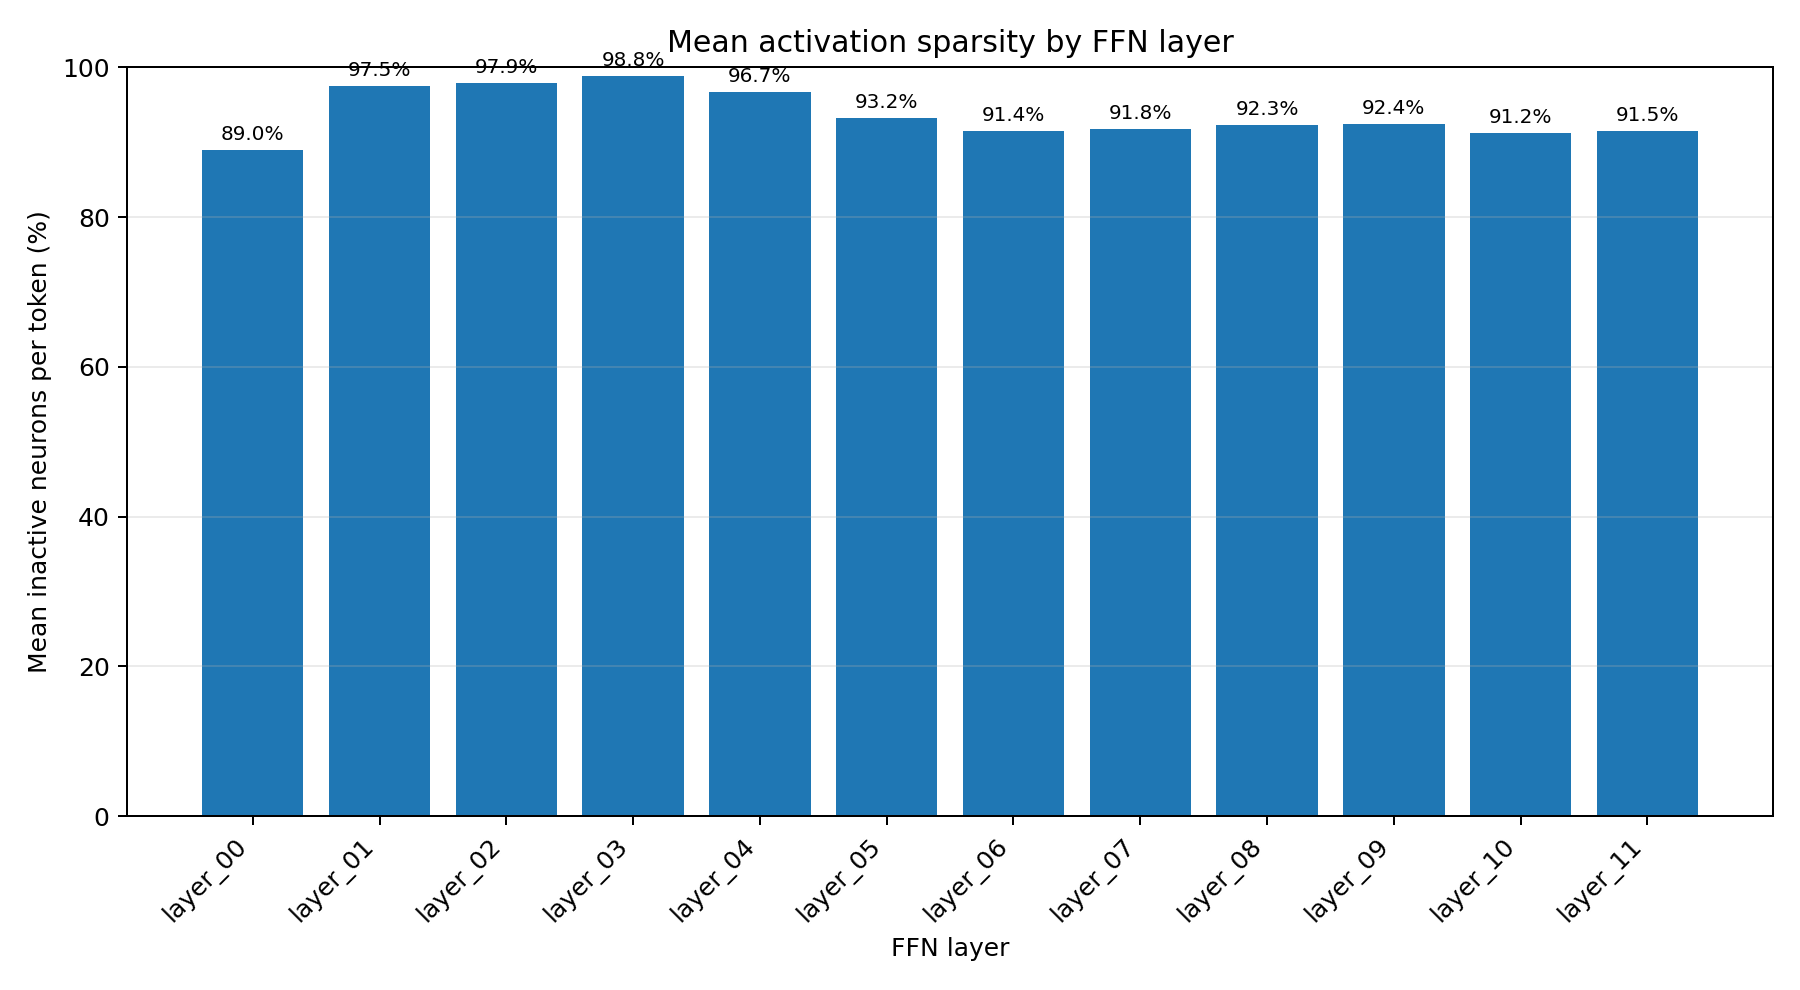
\includegraphics[width=0.88\textwidth]{figures/fig_layer_sparsity_bars.png}
    \caption{Mean token-wise exact-zero percentage across all 12 FFN layers of \texttt{facebook/opt-125m} on the WikiText-2 benchmark.}
    \label{fig:layer_sparsity_bars}
\end{figure}

The empirical measurements in Table~\ref{tab:phase1_descriptive} reveal three distinct behavioural phases across depth:
\begin{enumerate}
    \item \textbf{Input Filtering and Contraction (Layers~00--03):} Exact zero fractions rise from $88.96\%$ in Layer~00 to a global network maximum of $98.77\%$ in Layer~03. At Layer~03, an average of only $37.7$ coordinates out of $3{,}072$ fire per token, with the median coordinate firing probability dropping to $0.0586\%$. Simultaneously, token-to-token sparsity dispersion contracts 25-fold, from $\text{SD} = 0.0804$ at Layer~00 to $0.0032$ at Layer~03.
    \item \textbf{Intermediate Expansion and Plateau (Layers~05--10):} Sparsity stabilizes within a narrow band of $91.16\%\text{--}93.23\%$ ($208\text{--}272$ active units per token). Positive-tail skewness and excess kurtosis decrease markedly compared to early layers (skewness $1.88\text{--}2.30$, excess kurtosis $6.08\text{--}18.04$), while conditional positive activation amplitude increases monotonically from $0.1047$ to $0.2087$.
    \item \textbf{Terminal Broadening (Layer~11):} While sparsity remains at $91.49\%$, positive activation spread and tail heaviness increase substantially (positive mean $0.2517$, standard deviation $0.3145$, skewness $5.70$, and excess kurtosis $55.60$).
\end{enumerate}

The higher-order sample moments in Table~\ref{tab:phase1_descriptive} confirm severe non-normality at every layer, most notably at Layer~00 where sample excess kurtosis reaches $3{,}297.51$.

\section{RQ1: Profile Analysis of Layer-Wise Sparsity}

Figure~\ref{fig:rq1_profile} displays the block-averaged sparsity profile across all twelve layers for the $n = 40$ contiguous 128-token blocks, while Table~\ref{tab:rq1_tests} reports the formal multivariate and non-parametric hypothesis tests of profile flatness ($H_0 : \mat{C}\boldsymbol{\mu} = \vect{0}_{11}$).

\begin{figure}[htbp]
    \centering
    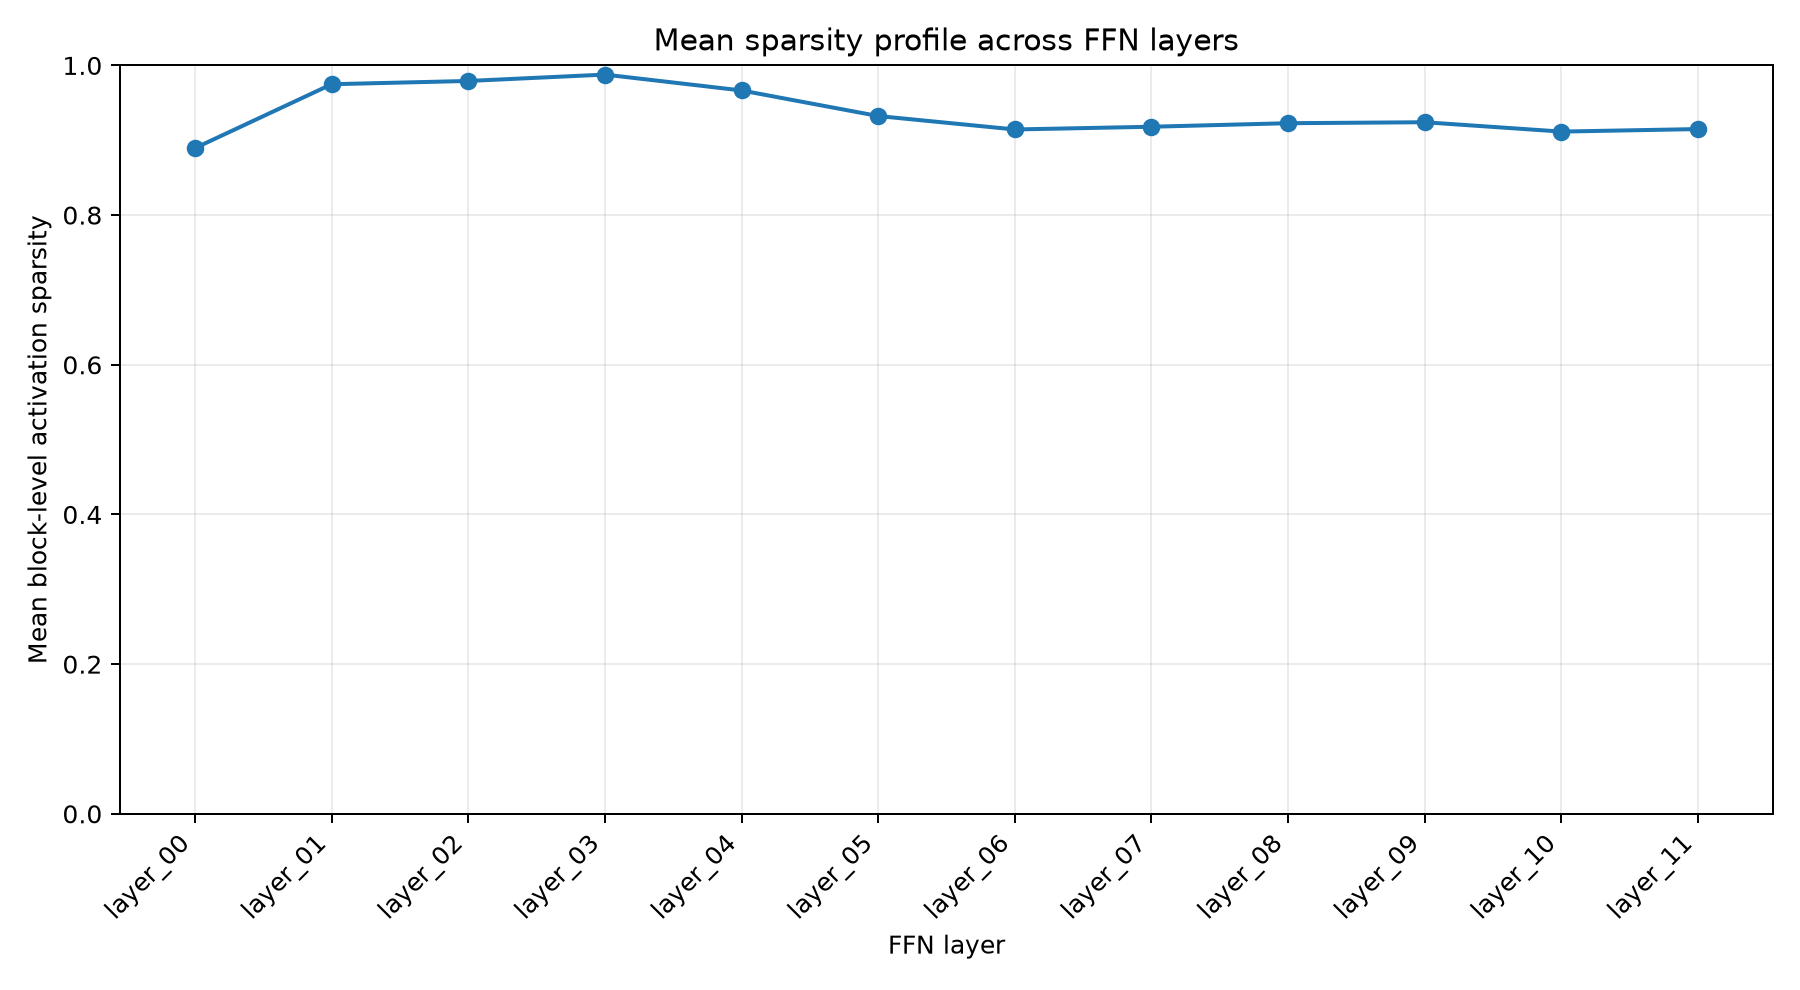
\includegraphics[width=0.88\textwidth]{figures/fig1_mean_sparsity_profile.png}
    \caption{Mean block-level activation sparsity profile across the 12 FFN layers ($n = 40$ blocks of 128 tokens). On the unit interval scale, the 95\% confidence intervals around each layer mean are narrower than the plot markers, demonstrating minimal block-to-block dispersion relative to depth-wise shifts.}
    \label{fig:rq1_profile}
\end{figure}

\begin{table}[htbp]
    \centering
    \caption{Multivariate and non-parametric hypothesis tests for layer-wise sparsity profile flatness (RQ1, $n = 40$ blocks, $q = 12$ layers).}
    \label{tab:rq1_tests}
    \small
    \begin{tabularx}{\textwidth}{@{}l l l l X@{}}
        \toprule
        \textbf{Test Procedure} & \textbf{Statistic} & \textbf{Degrees of Freedom} & \textbf{$p$-value} & \textbf{Decision} \\
        \midrule
        Hotelling's $T^2$ (Flatness) & $T^2 = 602{,}912.24$ & $F(11, 29) = 40{,}756.31$ & $1.25 \times 10^{-57}$ & Reject $H_0$ \\
        Repeated-Measures ANOVA & $F = 1{,}838.82$ & $\mathrm{df}_1 = 11,\; \mathrm{df}_2 = 429$ & $< 10^{-300}$ & Reject $H_0$ \\
        Greenhouse--Geisser ($\hat{\epsilon}=0.1253$) & $F = 1{,}838.82$ & $\mathrm{df}_1^* = 1.38,\; \mathrm{df}_2^* = 53.74$ & $1.68 \times 10^{-46}$ & Reject $H_0$ \\
        Friedman Rank Test & $Q = 432.99$ & $\mathrm{df} = 11$ & $5.99 \times 10^{-86}$ & Reject $H_0$ \\
        \bottomrule
    \end{tabularx}
\end{table}

In the repeated-measures sum-of-squares decomposition, variation attributable to layer depth ($SS_{\text{layers}} = 0.45200$) vastly exceeds both between-block variance ($SS_{\text{blocks}} = 0.00062$) and residual interaction error ($SS_{\text{error}} = 0.00959$). Because marginal variance at Layer~00 is considerably higher than at Layers~01--04, sphericity is severely violated ($\hat{\epsilon} = 0.1253$, approaching the theoretical lower bound of $1/11 = 0.0909$). Even after reducing numerator degrees of freedom from $11$ to $1.38$, the adjusted $F$-test rejects equal layer means at $p = 1.68 \times 10^{-46}$. Both Hotelling's $T^2$ (which is invariant to sphericity violations) and Friedman's rank test (which requires no normality assumption) corroborate this conclusion.

\section{RQ2: Binary Co-Activation Dependence and Hierarchical Clustering}

Applying the prevalence filter~\eqref{eq:prevalence_filter} ($0.01 \le \hat{\pi}_k \le 0.99$) demonstrates substantial depth heterogeneity in the count of non-degenerate coordinates. Table~\ref{tab:rq2_all_layers} presents the binary dependence metrics across all twelve layers on the $m = 128$ sampled coordinates, while Figures~\ref{fig:rq2_phi_heatmaps} and~\ref{fig:rq2_dendrogram} illustrate the structural transition from Layer~00 to Layer~06.

\begin{table}[htbp]
    \centering
    \caption{Binary co-activation dependence metrics across all 12 layers (RQ2, $M = 5{,}120$ tokens, $m = 128$ sampled coordinates from $\mathcal{K}_{\text{elig}}^{(\ell)}$, average-linkage cluster cutoff $d = 1 - \phi = 0.70$).}
    \label{tab:rq2_all_layers}
    \small
    \setlength{\tabcolsep}{8pt}
    \begin{tabular}{@{}l c r r c c@{}}
        \toprule
        \textbf{Layer} & \textbf{Eligible Units} & \textbf{Mean $\phi$} & \textbf{Median $\phi$} & \textbf{Positive Pairs (\%)} & \textbf{Clusters ($d = 0.70$)} \\
        \midrule
        Layer 00 & 3008 & 0.0685 &  0.0422 & 76.82 &  94 \\
        Layer 01 &  624 & 0.0067 & $-0.0116$ & 37.01 &  92 \\
        Layer 02 &  719 & 0.0054 & $-0.0112$ & 38.57 & 106 \\
        Layer 03 &  536 & 0.0034 & $-0.0113$ & 37.33 & 112 \\
        Layer 04 & 1081 & 0.0059 & $-0.0082$ & 41.20 & 108 \\
        Layer 05 & 1810 & 0.0028 & $-0.0067$ & 42.47 & 118 \\
        Layer 06 & 2184 & 0.0042 & $-0.0047$ & 45.14 & 122 \\
        Layer 07 & 2312 & 0.0026 & $-0.0066$ & 43.44 & 121 \\
        Layer 08 & 2445 & 0.0034 & $-0.0078$ & 43.02 & 114 \\
        Layer 09 & 2602 & 0.0036 & $-0.0089$ & 40.31 & 112 \\
        Layer 10 & 2690 & 0.0071 & $-0.0073$ & 43.63 & 111 \\
        Layer 11 & 2732 & 0.0391 &  0.0115 & 57.28 &  94 \\
        \bottomrule
    \end{tabular}
\end{table}

\begin{figure}[htbp]
    \centering
    \begin{minipage}{0.48\textwidth}
        \centering
        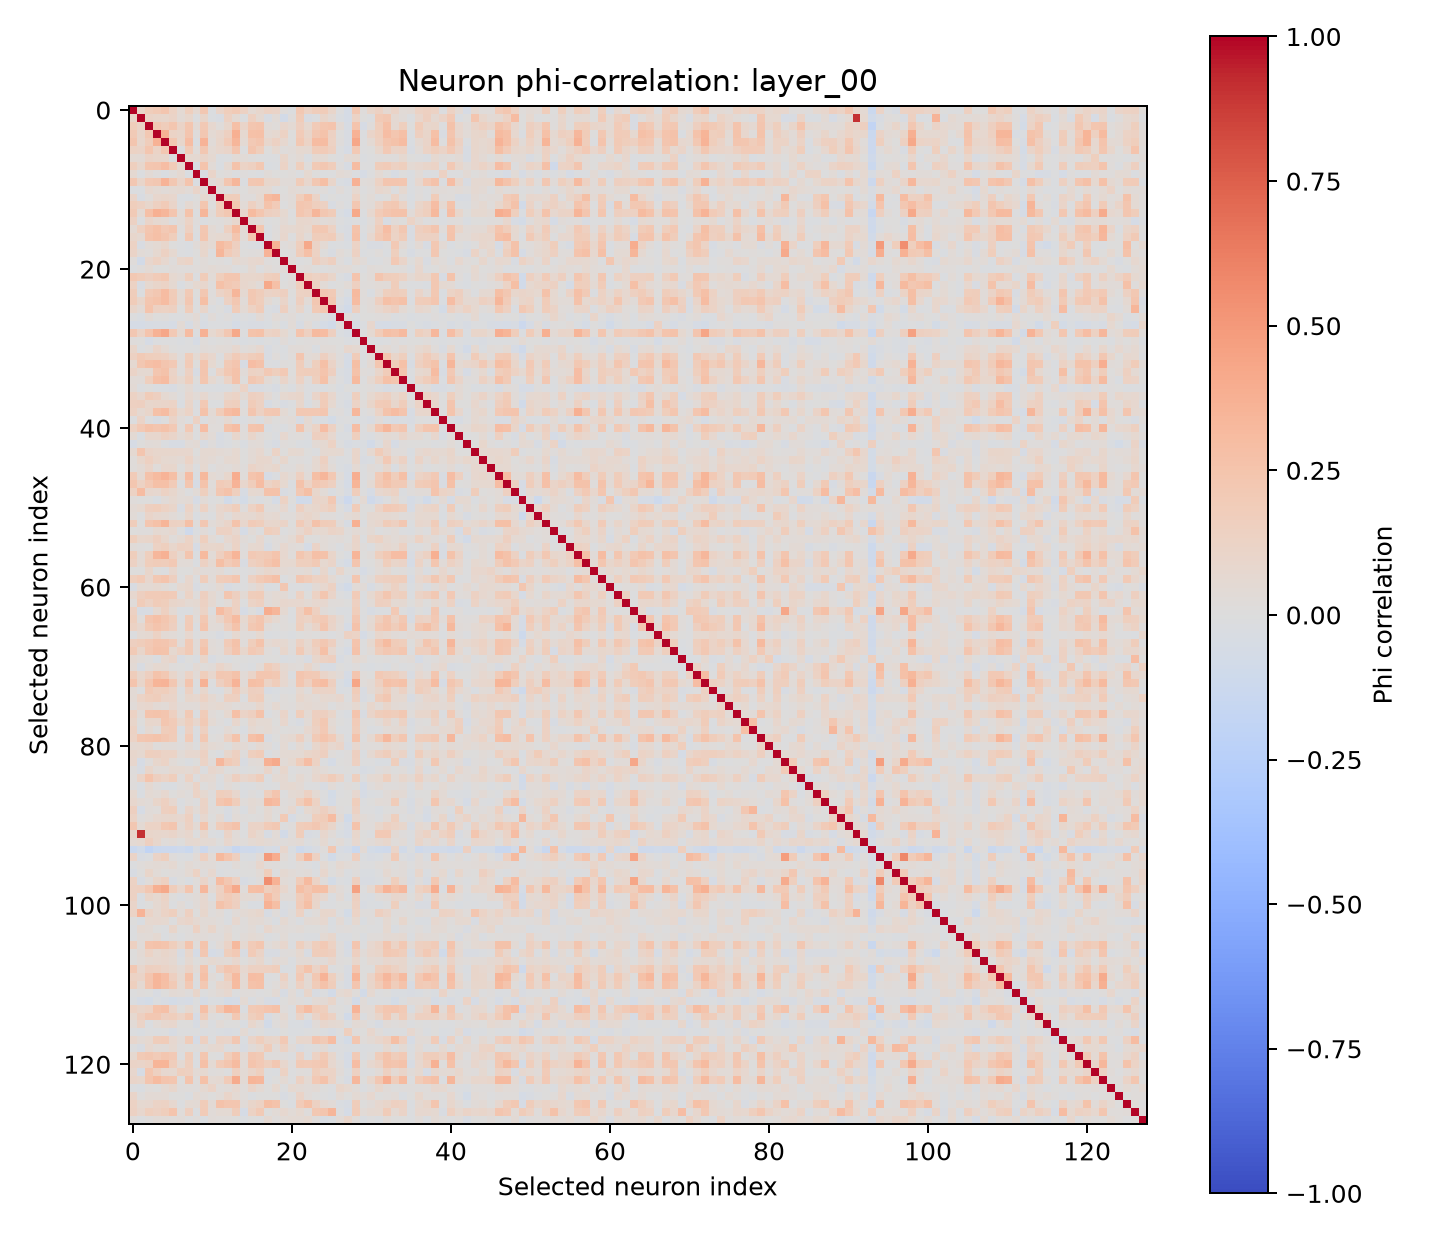
\includegraphics[width=\linewidth]{figures/fig2a_phi_corr_l00.png}
        \caption*{(a) Layer 00 $\phi$-Correlation Matrix}
    \end{minipage}\hfill
    \begin{minipage}{0.48\textwidth}
        \centering
        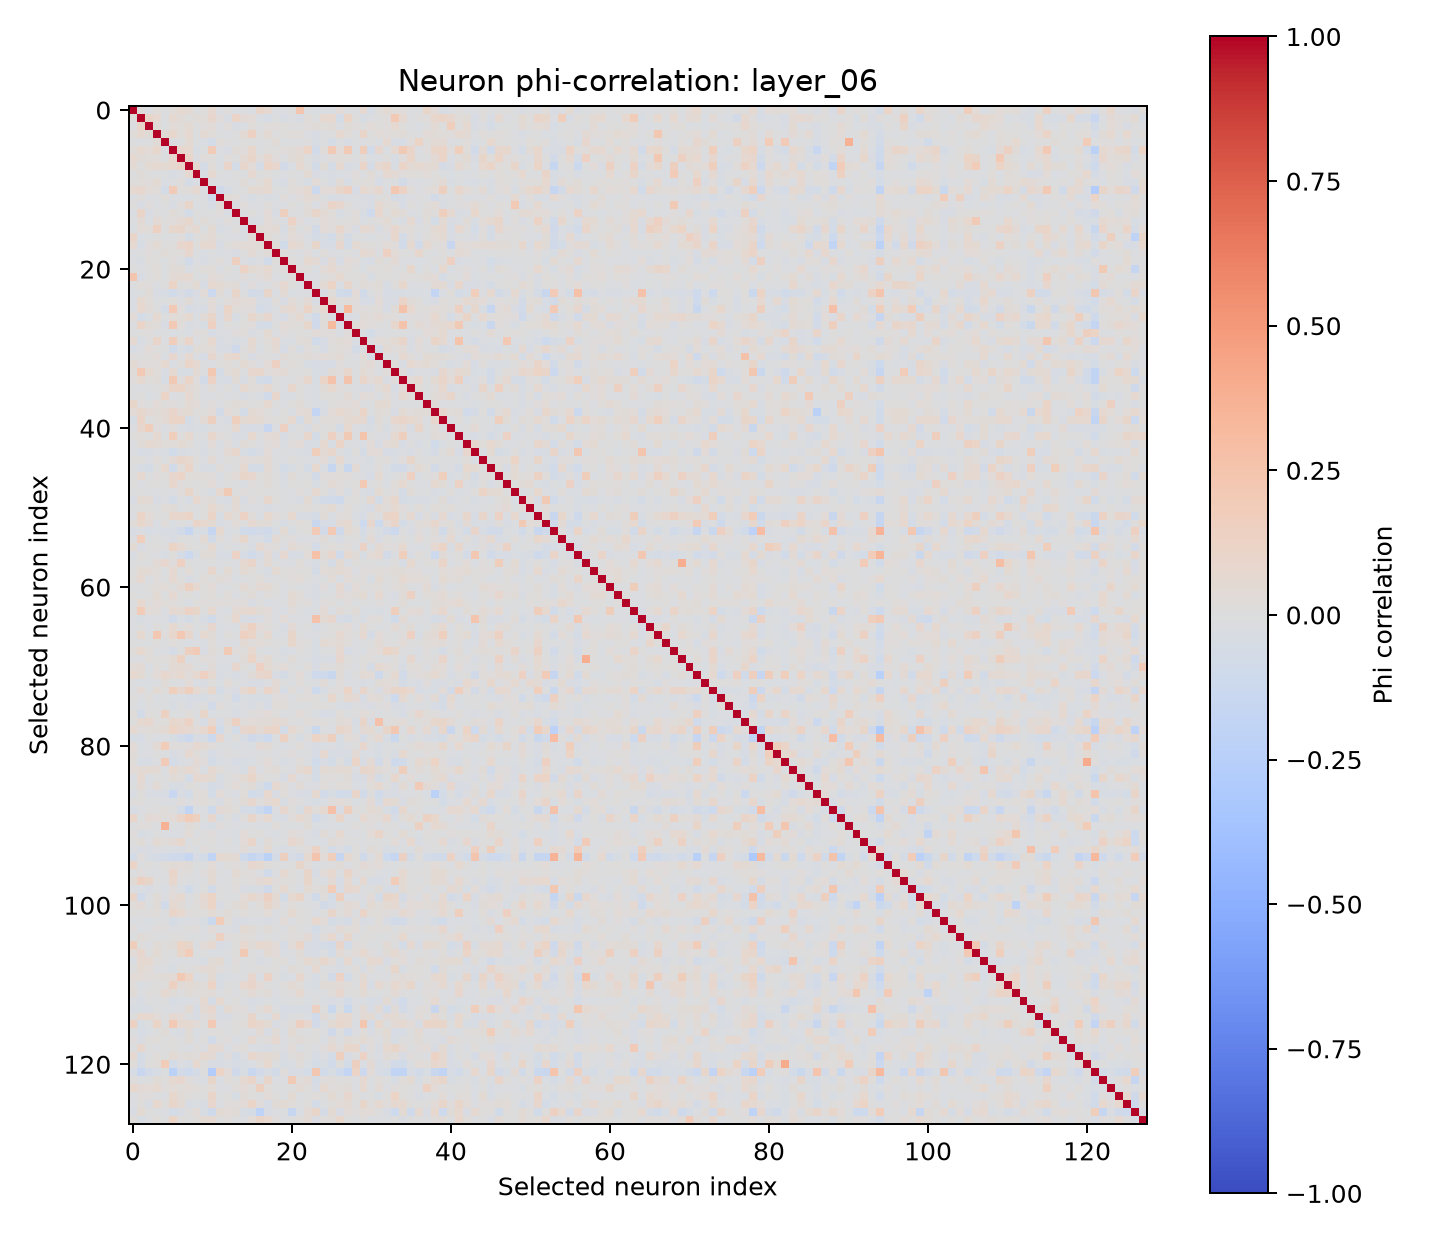
\includegraphics[width=\linewidth]{figures/fig2b_phi_corr_l06.png}
        \caption*{(b) Layer 06 $\phi$-Correlation Matrix}
    \end{minipage}
    \caption{Pairwise binary $\phi$-correlation heatmaps on $m = 128$ prevalence-filtered coordinates: (a) Layer~00 exhibits broad positive co-activation, whereas (b) Layer~06 displays near-complete pairwise decorrelation.}
    \label{fig:rq2_phi_heatmaps}
\end{figure}

\begin{figure}[htbp]
    \centering
    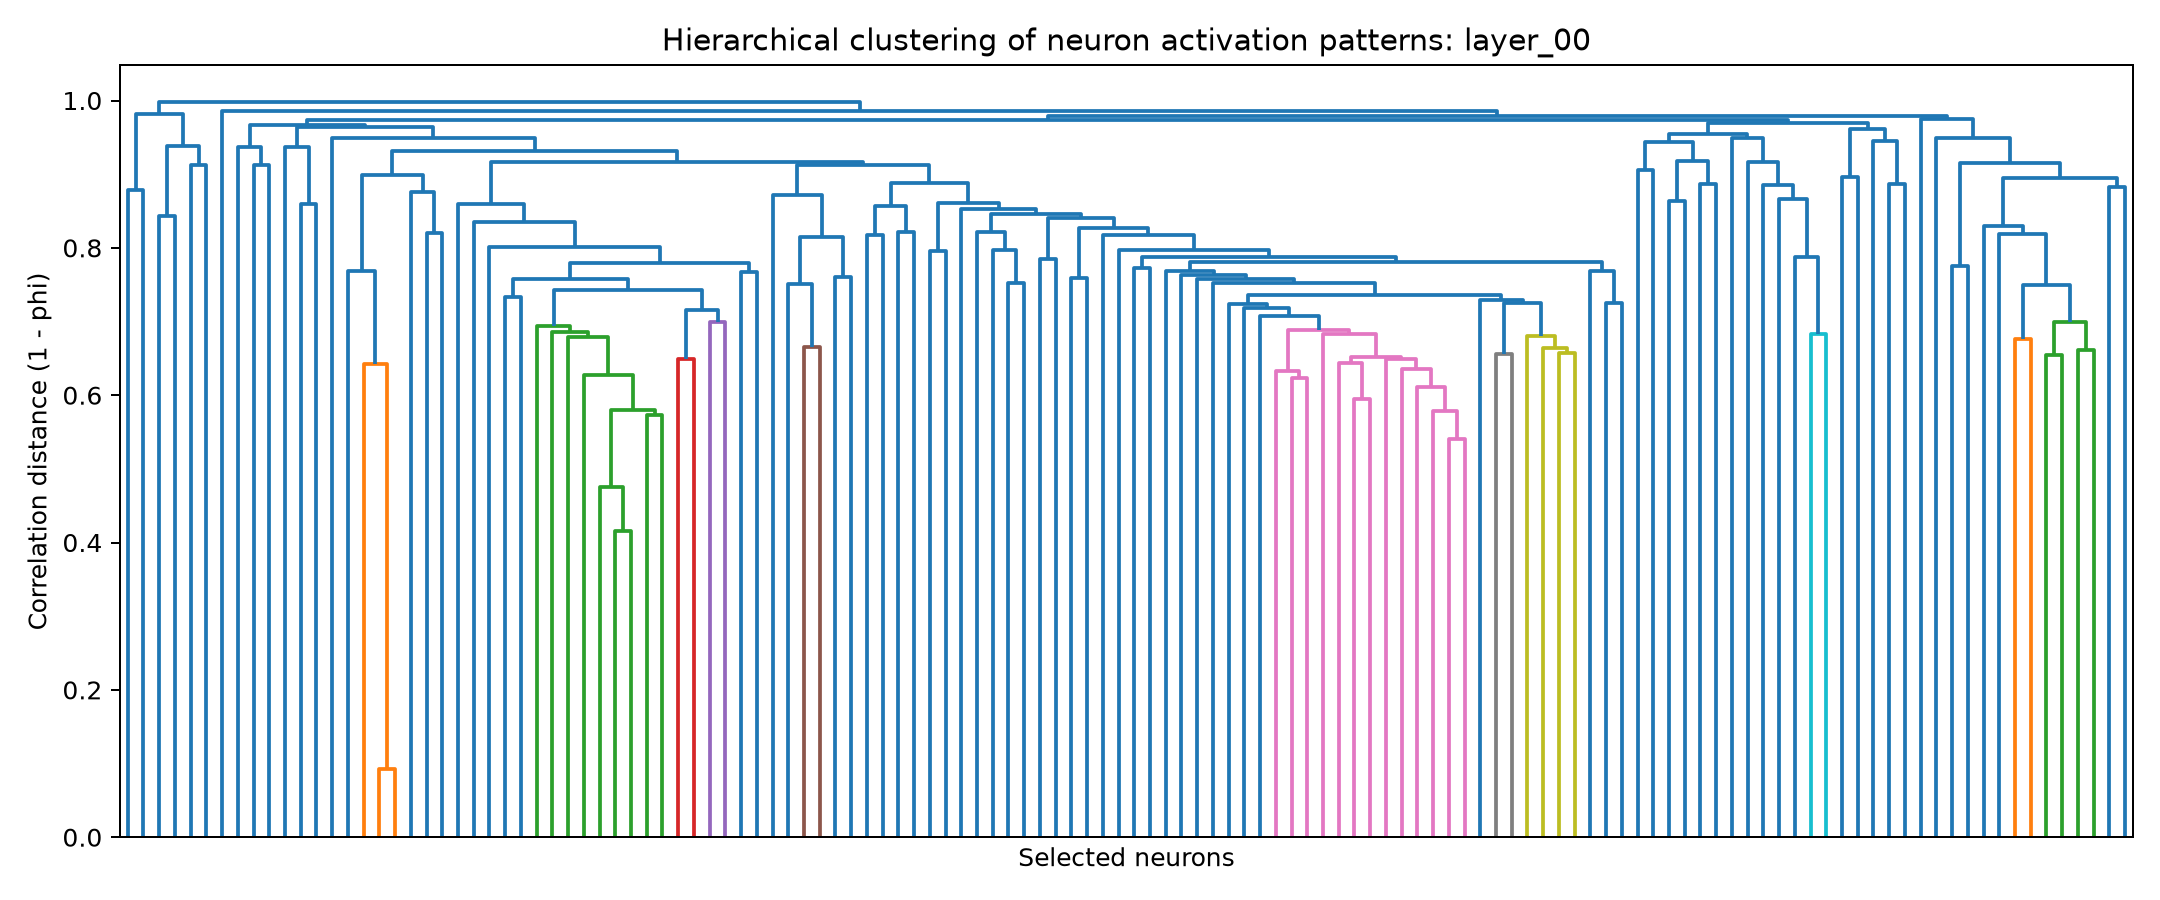
\includegraphics[width=0.82\textwidth]{figures/fig2c_dendrogram_l00.png}
    \caption{Hierarchical agglomerative clustering dendrogram (average linkage, dissimilarity $d_{jk} = 1 - \phi_{jk}$) for 128 sampled coordinates in Layer~00. Coherent clusters emerge below $d = 0.70$, including an isolated pair at $d \approx 0.09$ ($\phi \approx 0.91$) and multi-unit groups of approximately 8 and 11 coordinates.}
    \label{fig:rq2_dendrogram}
\end{figure}

A comprehensive analysis across all twelve layers reveals a non-monotonic, U-shaped trajectory of binary co-activation dependence:
\begin{itemize}
    \item \textbf{Layer~00 (Co-Activated Input Stage):} Nearly all coordinates satisfy prevalence criteria ($3{,}008$ out of $3{,}072$). Over three-quarters of pairs ($76.82\%$) exhibit positive correlation ($\bar{\phi} = 0.0685$, median $0.0422$), visible in Figure~\ref{fig:rq2_phi_heatmaps}(a) as a consistent positive off-diagonal background with isolated strongly coupled pairs ($\phi \approx 0.91$). Average-linkage clustering (Figure~\ref{fig:rq2_dendrogram}) partitions the $128$ coordinates into $94$ clusters at $d = 0.70$, featuring tight sub-clusters merging between $d = 0.09$ and $0.70$.
    \item \textbf{Layers~01--10 (Decorrelated Interior Processing):} Eligible units decline to $536$ in Layer~03 before recovering to $2{,}690$ in Layer~10. Across these interior layers, mean pairwise $\phi$ drops near zero ($0.0026\text{--}0.0071$), median $\phi$ becomes slightly negative ($-0.0116$ to $-0.0047$), and cluster counts peak at $122$ out of $128$ at Layer~06, reflecting the near-neutral background in Figure~\ref{fig:rq2_phi_heatmaps}(b).
    \item \textbf{Layer~11 (Terminal Re-Coupling):} Positive co-activation re-emerges ($\bar{\phi} = 0.0391$, median $0.0115$, $57.28\%$ positive pairs), returning the cluster count to $94$.
\end{itemize}

\section{RQ3: Latent Dimensionality, Subspace Stability, and Factor Diagnostics}

Table~\ref{tab:rq3_dimensionality} summarizes the covariance PCA effective dimensionality metrics, reconstruction errors, and split-half subspace stability across all twelve layers. Figure~\ref{fig:rq3_scree} compares the eigenvalue scree plots and cumulative variance profiles of Layer~00 and Layer~06.

\begin{table}[htbp]
    \centering
    \caption{Layer-wise covariance PCA effective dimensionality, reconstruction error, and split-half principal-angle stability (RQ3, $N = 5{,}000$ tokens per layer).}
    \label{tab:rq3_dimensionality}
    \small
    \setlength{\tabcolsep}{8pt}
    \begin{tabular}{@{}l r r c r r@{}}
        \toprule
        \textbf{Layer} & \textbf{PR} & \textbf{Entropy $\erank$} & \textbf{$K$ for 80\% Var.} & \textbf{Recon.\ Error ($K=10$)} & \textbf{Split-Half $\bar{\rho}_{10}$} \\
        \midrule
        Layer 00 &  1.12 &  1.51 &    1   & 0.0788 & 0.941 \\
        Layer 01 &  3.89 & 13.06 & $>64$  & 0.4692 & 0.939 \\
        Layer 02 &  1.20 &  1.86 &    1   & 0.1125 & 0.918 \\
        Layer 03 &  2.45 &  7.72 & $>64$  & 0.3861 & 0.968 \\
        Layer 04 &  3.51 & 12.19 & $>64$  & 0.4927 & 0.948 \\
        Layer 05 & 31.40 & 46.36 & $>64$  & 0.7917 & 0.914 \\
        Layer 06 & 29.86 & 45.53 & $>64$  & 0.7911 & 0.878 \\
        Layer 07 & 30.99 & 45.98 & $>64$  & 0.7977 & 0.898 \\
        Layer 08 & 31.42 & 46.10 & $>64$  & 0.7933 & 0.919 \\
        Layer 09 & 29.64 & 44.03 & $>64$  & 0.7744 & 0.885 \\
        Layer 10 & 27.64 & 41.43 & $>64$  & 0.7212 & 0.913 \\
        Layer 11 &  3.38 & 10.81 & $>64$  & 0.3978 & 0.941 \\
        \bottomrule
    \end{tabular}
\end{table}

\begin{figure}[htbp]
    \centering
    \begin{minipage}{0.48\textwidth}
        \centering
        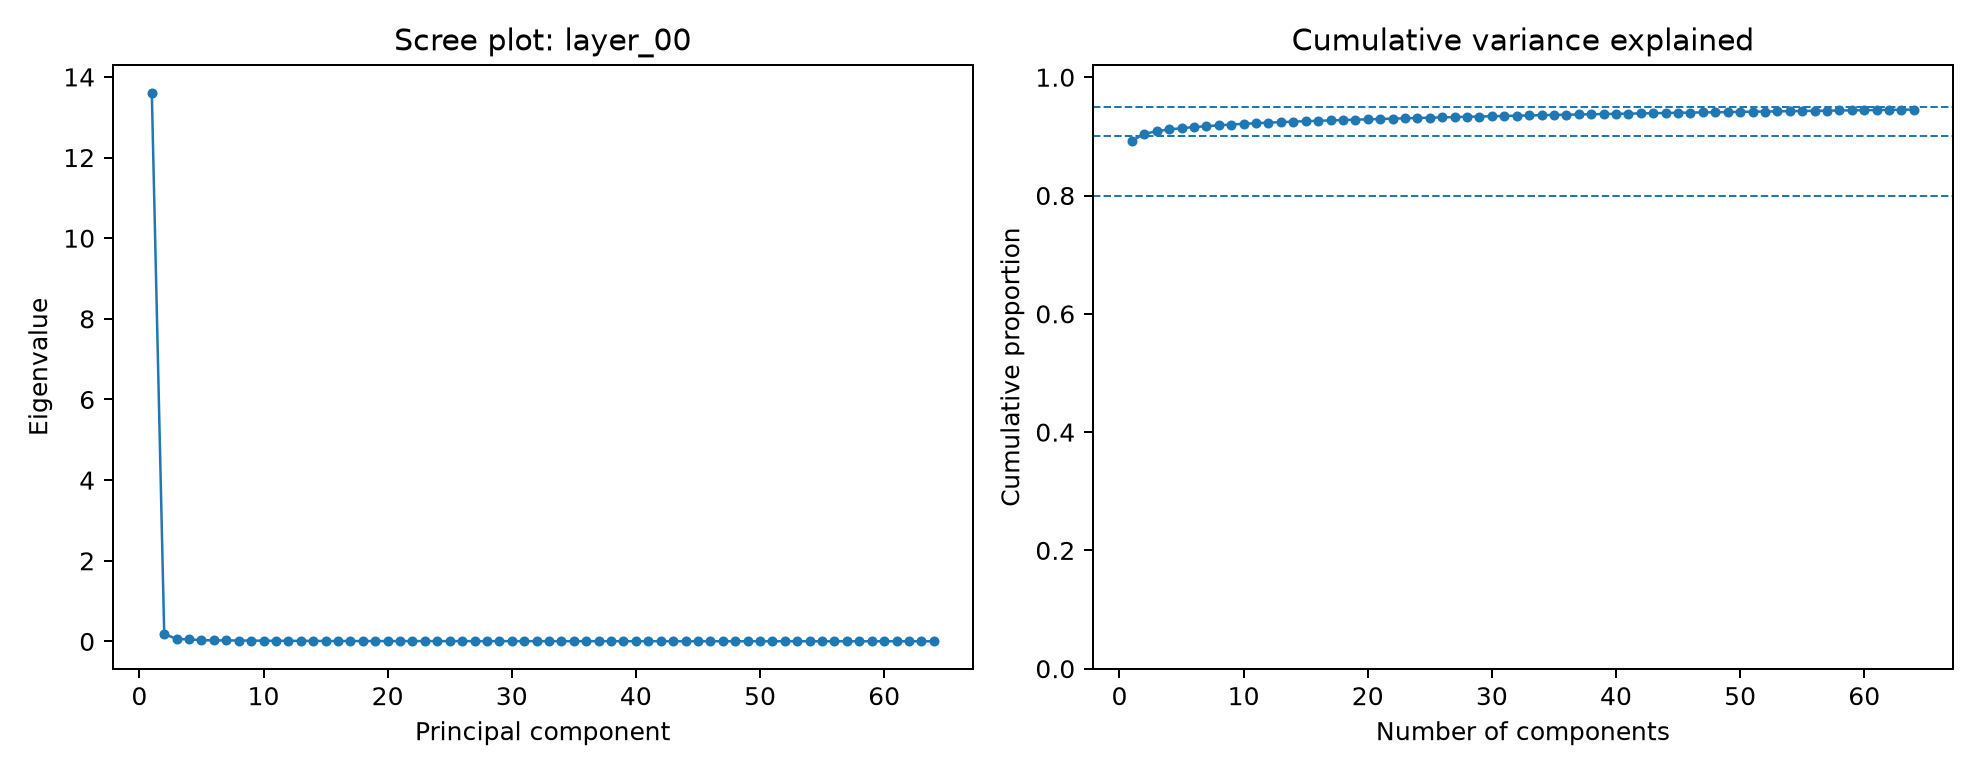
\includegraphics[width=\linewidth]{figures/fig3a_pca_scree_l00.png}
        \caption*{(a) Layer 00 Eigenvalues and Cumulative Variance}
    \end{minipage}\hfill
    \begin{minipage}{0.48\textwidth}
        \centering
        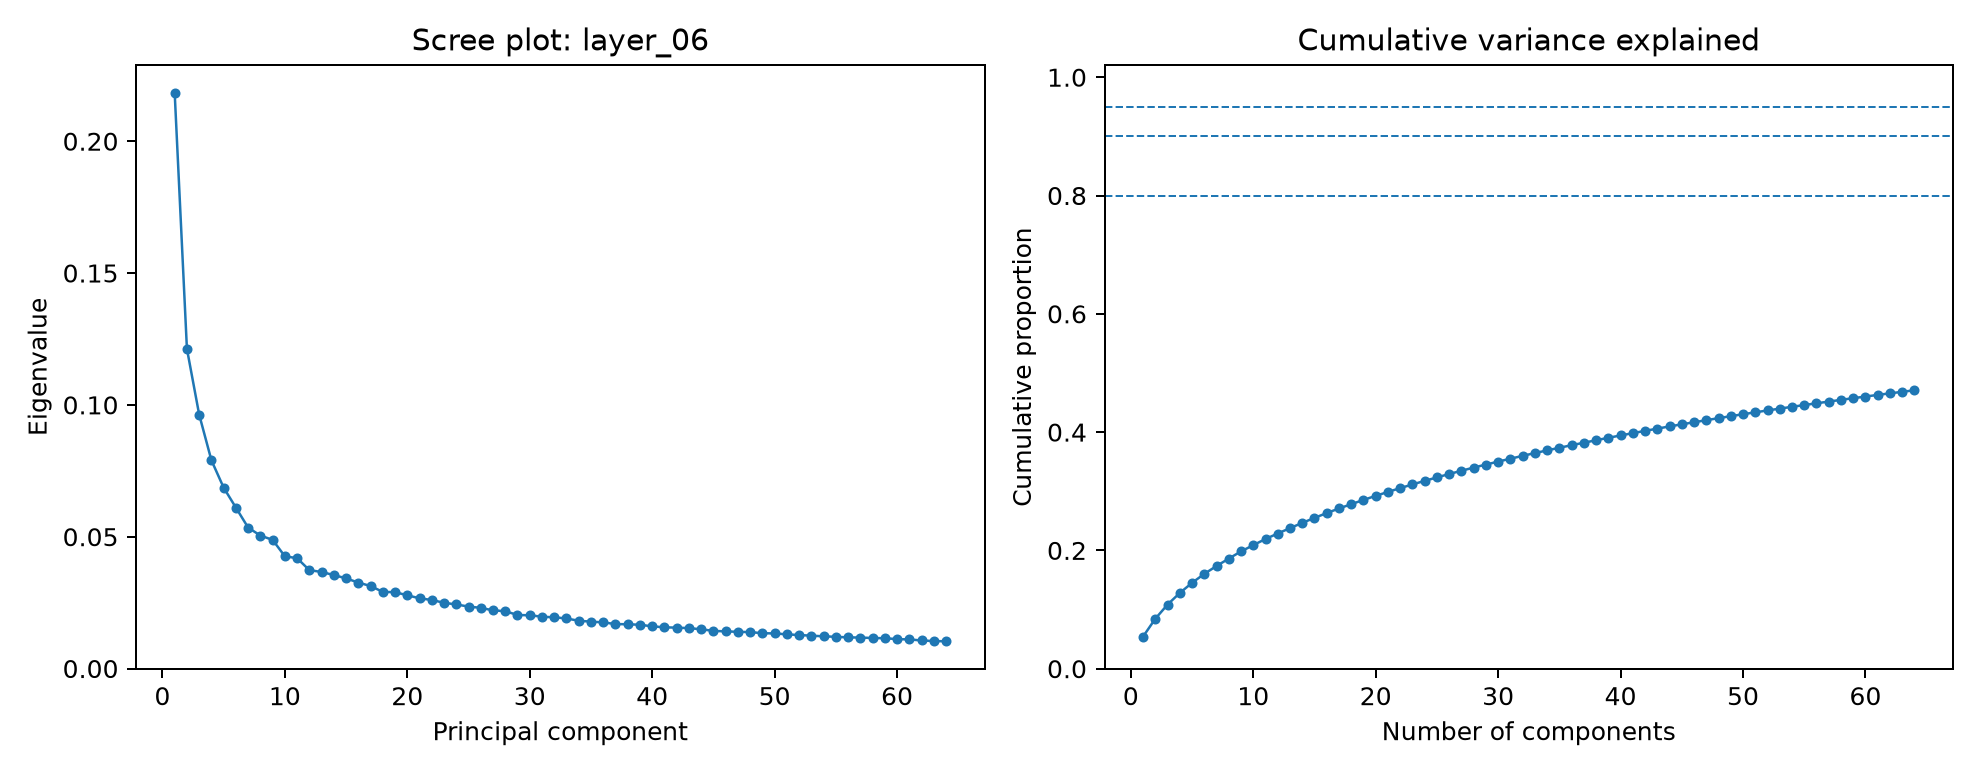
\includegraphics[width=\linewidth]{figures/fig3b_pca_scree_l06.png}
        \caption*{(b) Layer 06 Eigenvalues and Cumulative Variance}
    \end{minipage}
    \caption{Covariance PCA eigenvalue scree plots and cumulative variance curves: (a) Layer~00 displays acute low-rank collapse ($\hat{\lambda}_1 \approx 13.6$ vs.\ $\hat{\lambda}_2 \approx 0.16$, where PC1 captures $\approx 89\%$ of total variance), while (b) Layer~06 displays an expanded spectrum requiring $>64$ components to reach $80\%$ variance.}
    \label{fig:rq3_scree}
\end{figure}

The empirical spectra exhibit three prominent structural characteristics:
\begin{enumerate}
    \item \textbf{Acute Low-Rank Collapse in Layers~00 and~02:} In Layer~00 ($\PR = 1.12$, $\erank = 1.51$), the first eigenvalue $\hat{\lambda}_1 \approx 13.6$ exceeds the second eigenvalue $\hat{\lambda}_2 \approx 0.16$ by a factor of $85$. PC1 accounts for approximately $89\%$ of total covariance trace, and cumulative variance reaches $94.5\%$ at $K = 64$. Layer~02 displays similar collapse ($\PR = 1.20$, $\erank = 1.86$), with $K = 10$ components leaving only $7.88\%$ and $11.25\%$ unexplained variance in Layers~00 and~02, respectively.
    \item \textbf{Mid-Network Spectral Expansion (Layers~05--10):} Effective dimensionality increases substantially to $\erank \in [41.43, 46.36]$ ($\PR \in [27.64, 31.42]$). In Layer~06 (Figure~\ref{fig:rq3_scree}(b)), eigenvalues decay slowly ($\hat{\lambda}_1 \approx 0.217$, $\hat{\lambda}_2 \approx 0.121$, $\hat{\lambda}_3 \approx 0.096$), such that $K = 10$ components capture only $20.9\%$ of total variance, and even $K = 64$ captures merely $\approx 47\%$.
    \item \textbf{Terminal Compression and Subspace Reproducibility:} At Layer~11, effective rank decreases to $\erank = 10.81$ ($\PR = 3.38$). Across all twelve layers, split-half mean principal-angle cosines at $K = 10$ remain between $0.878$ and $0.968$, confirming that estimated principal subspaces are statistically stable across independent token splits.
\end{enumerate}

\subsection{Sampling Adequacy and Factor Analysis Diagnostics}

Figure~\ref{fig:rq3_factor_loadings} presents the Varimax-rotated factor loading heatmap for an exploratory $K = 5$ Gaussian factor model fitted on $m = 256$ prevalence-filtered coordinates in Layer~00. Loading magnitudes are concentrated near zero across nearly all entries, with sparse isolated bands reaching $+0.02$ to $+0.035$ (primarily on $F_2$, and narrow spikes on $F_3$ near indices $110$ and $125$), and a negative band near $-0.015$. This attenuation directly reflects the low marginal variances induced by $88.96\%$ zero-inflation. In interior layers where pairwise correlations approach zero, sample correlation matrices approximate $\mat{I}_m$, lowering the KMO index~\eqref{eq:kmo_def} and reducing common-factor identifiability. Consequently, covariance PCA provides an objective, distribution-free decomposition of variance geometry, whereas Gaussian factor models serve primarily as diagnostic tools highlighting non-normality.

\begin{figure}[htbp]
    \centering
    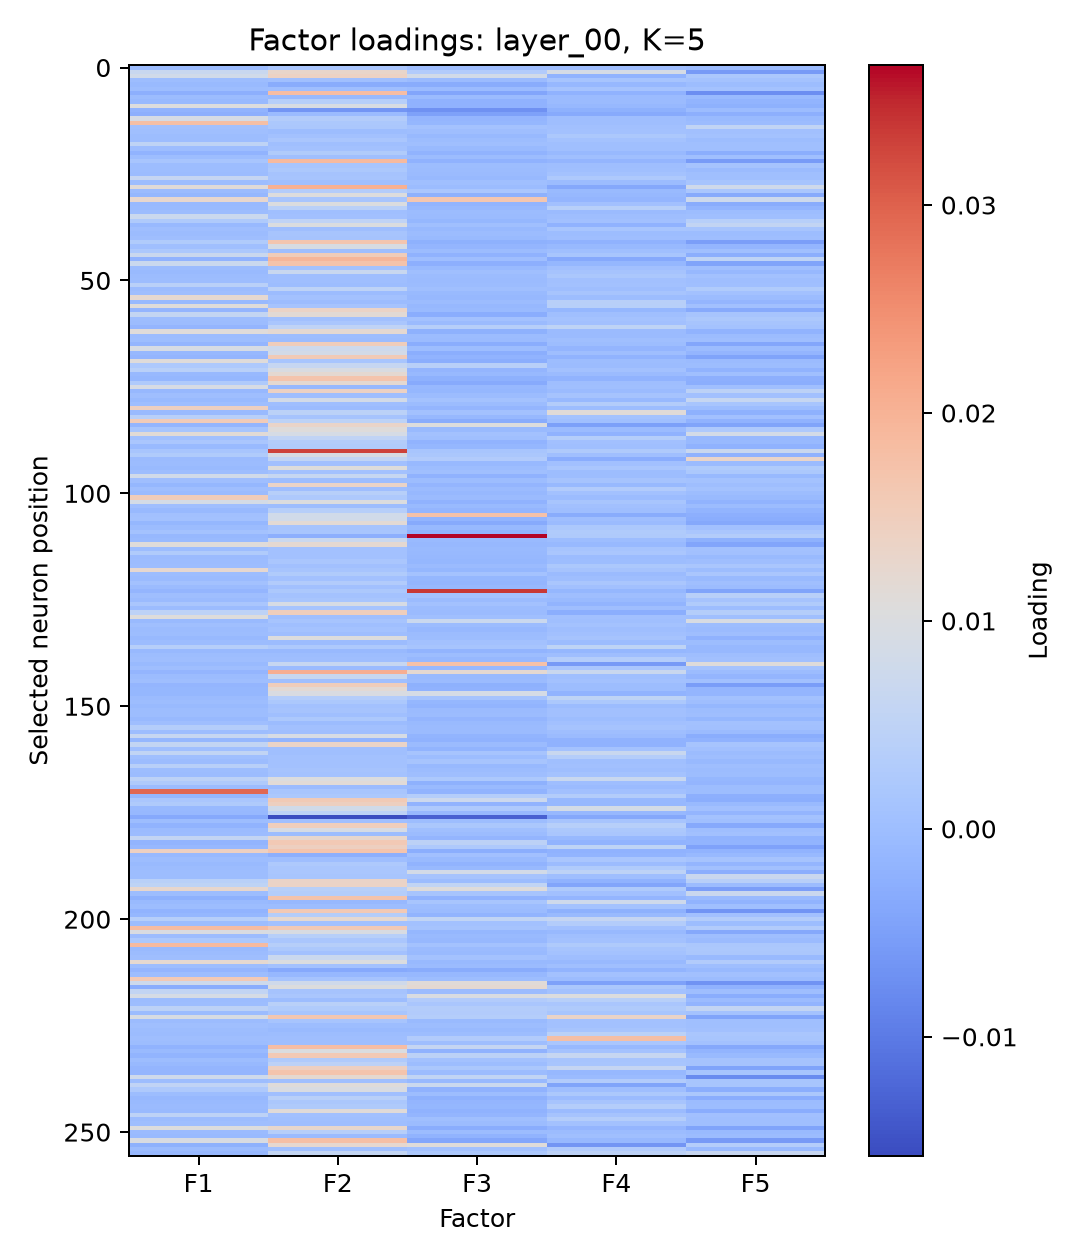
\includegraphics[width=0.72\textwidth]{figures/fig3c_factor_loadings_l00.png}
    \caption{Exploratory Varimax-rotated Gaussian factor loading heatmap for $m = 256$ coordinates in Layer~00 ($K = 5$ factors). Near-zero background loadings with sparse spikes reflect low marginal variances under severe zero-inflation.}
    \label{fig:rq3_factor_loadings}
\end{figure}

\section{RQ4: Empirical Activation Rank versus Actual Weight Matrix SVD}

Singular value decomposition of the actual parameter matrices (\texttt{fc1} and \texttt{fc2}) from \texttt{facebook/opt-125m} yields an average weight entropy effective rank of $\overline{\erank}_W = 500.53$ ($\overline{\PR}_W = 281.52$), compared with an average empirical activation effective rank of $\overline{\erank}_A = 26.38$ ($\overline{\PR}_A = 16.38$). Table~\ref{tab:rq4_corr} reports layer-wise rank association statistics, Figure~\ref{fig:rq4_weights} illustrates singular spectra and depth profiles, and Appendix Table~\ref{tab:app_rq4_layer_data} lists the complete layer-by-layer values.

\begin{table}[htbp]
    \centering
    \caption{Cross-layer association between empirical activation effective dimensionality and actual \texttt{facebook/opt-125m} weight matrix spectral dimensionality (RQ4, $n = 12$ layers).}
    \label{tab:rq4_corr}
    \footnotesize
    \begin{tabularx}{\textwidth}{@{}l r r X@{}}
        \toprule
        \textbf{Metric Comparison} & \textbf{Correlation} & \textbf{$p$-value} & \textbf{Statistical Inference ($\alpha = 0.05$)} \\
        \midrule
        Pearson $r$ (Entropy Effective Rank) & $+0.7991$ & $0.00182$ & Statistically significant positive association \\
        Spearman $\rho$ (Entropy Effective Rank) & $+0.8392$ & $0.00064$ & Statistically significant monotone coupling \\
        Pearson $r$ (Participation Ratio) & $+0.8432$ & $0.00057$ & Statistically significant positive association \\
        Spearman $\rho$ (Participation Ratio) & $+0.7622$ & $0.00395$ & Statistically significant monotone coupling \\
        \bottomrule
    \end{tabularx}
\end{table}

\begin{figure}[htbp]
    \centering
    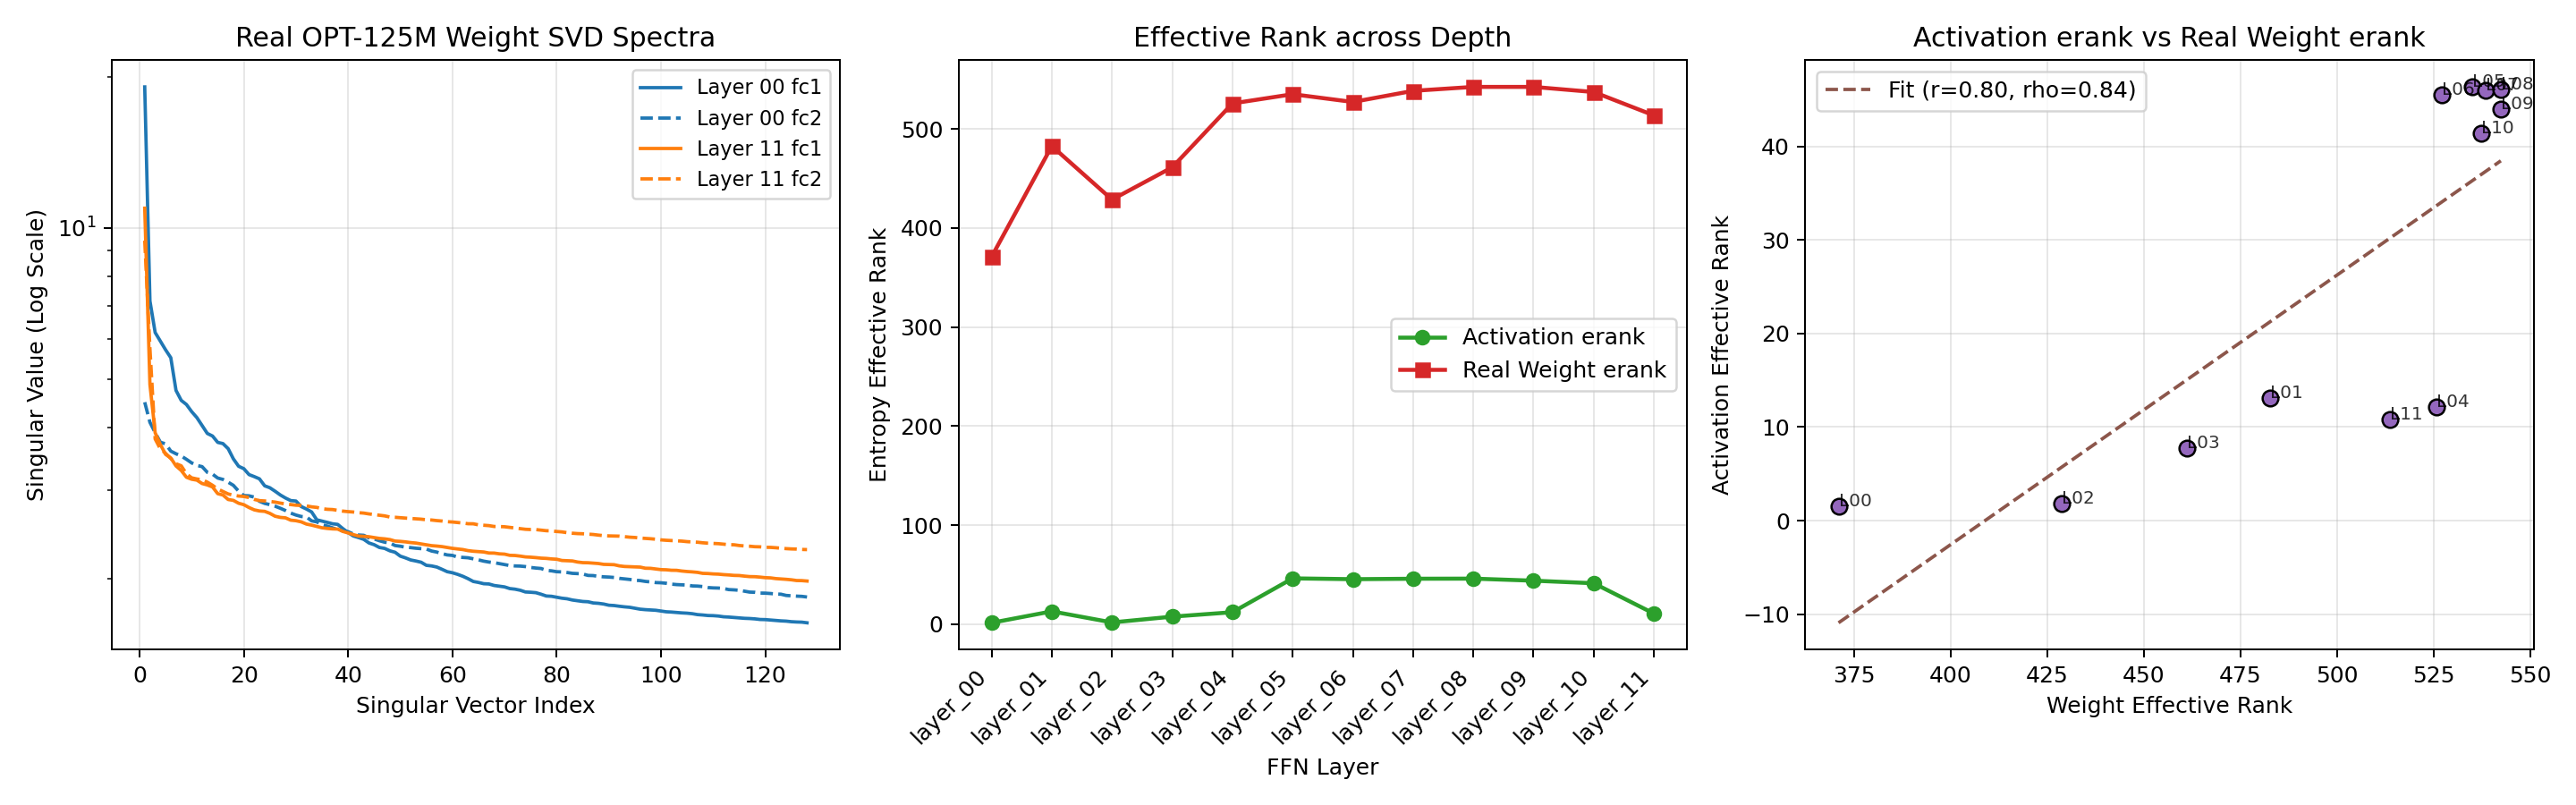
\includegraphics[width=0.95\textwidth]{figures/fig4_activation_vs_weight_rank.png}
    \caption{Comparison of empirical activation effective rank and real \texttt{facebook/opt-125m} FFN weight matrix SVD spectra across depth: (left) top 128 singular values of \texttt{fc1} and \texttt{fc2} on logarithmic scale, (centre) depth-wise effective rank trajectories, and (right) scatter plot of activation rank versus weight rank ($r = 0.80$, $\rho = 0.84$).}
    \label{fig:rq4_weights}
\end{figure}

Two principal statistical insights emerge from Table~\ref{tab:rq4_corr} and Figure~\ref{fig:rq4_weights}:
\begin{enumerate}
    \item \textbf{Positive Depth Coupling and Two-Regime Structure:} Contrary to the assumption that weight spectra are uniform across depth, actual parameter matrices exhibit pronounced spectral contraction in early layers. In Figure~\ref{fig:rq4_weights} (left), Layer~00 \texttt{fc1} exhibits a steep leading singular value ($s_1 > 20$) followed by rapid decay, resulting in the lowest weight effective ranks in the network (Layer~00: \texttt{fc1} $\erank = 232.38$, $\PR = 28.63$, mean $\erank_W = 371.04$; Layer~02: \texttt{fc1} $\erank = 310.96$, mean $\erank_W = 428.70$). These correspond directly to the layers where empirical activation rank collapses ($\erank_A = 1.51$ and $1.86$). In middle layers (Layers~05--10), mean weight rank plateaus at $527.24\text{--}542.47$ concurrent with activation expansion ($\erank_A \in [41.43, 46.36]$). Because the scatter plot (Figure~\ref{fig:rq4_weights}, right) partitions into early/terminal layers versus a distinct mid-depth cluster, the non-parametric Spearman rank correlation ($\rho = 0.839$, $p = 0.00064$) provides a robust measure of monotonic coupling alongside Pearson's linear coefficient ($r = 0.799$, $p = 0.0018$).
    \item \textbf{Scale Discrepancy Between Operator Capacity and Dynamic Response:} Despite strong relative depth correlation, absolute activation effective rank ($\overline{\erank}_A = 26.38$) remains roughly 19 times smaller than mean weight effective rank ($\overline{\erank}_W = 500.53$) and nearly 30 times below the algebraic rank limit ($768$). Static parameter spectra establish relative structural capacity across depth, while non-linear ReLU gating and input geometry govern dynamic rank compression.
\end{enumerate}

\section{RQ5: Cross-Domain Representation Stability and Discriminant Analysis}

To test representation invariance across linguistic populations, $N = 3{,}000$ genuine tokens ($1{,}000$ each from Wikipedia, ML-ArXiv scientific abstracts, and AG-News) were extracted from Layer~00 and projected onto $K = 8$ common principal components. Table~\ref{tab:rq5_tests} reports multivariate test statistics and classification metrics, while Figure~\ref{fig:rq5_lda} displays the two-dimensional canonical discriminant projection.

\begin{table}[htbp]
    \centering
    \caption{Multivariate hypothesis tests and 5-fold cross-validated classification performance across three genuine text corpora in Layer~00 (RQ5, $N = 3{,}000$, $G = 3$, $K = 8$ principal components).}
    \label{tab:rq5_tests}
    \small
    \setlength{\tabcolsep}{6pt}
    \begin{tabular}{@{}l r l r l@{}}
        \toprule
        \textbf{Test / Classifier} & \textbf{Value} & \textbf{Test Statistic / Details} & \textbf{$p$-value} & \textbf{Inference} \\
        \midrule
        MANOVA: Wilks' $\Lambda$ & $0.6939$ & Rao $F(16, 5980) = 74.94$ & $7.86 \times 10^{-223}$ & Reject equal centroids \\
        MANOVA: Pillai's Trace & $0.3208$ & $s = 2$ non-zero roots & $< 10^{-200}$ & Reject equal centroids \\
        MANOVA: Hotelling--Lawley & $0.4201$ & $\sum \xi_r = 0.4201$ & $< 10^{-200}$ & Reject equal centroids \\
        MANOVA: Roy's Root & $\xi_1 = 0.3619$ & $\theta = 0.2657$ ($s=2, \tilde{n}=1494$) & $< 10^{-200}$ & Reject equal centroids \\
        Box's $M$ Test & $8{,}164.09$ & $\chi^2(72) = 8{,}133.62$ & $< 10^{-300}$ & Reject equal covariances \\
        \midrule
        $T^2$: Wiki vs.\ Sci & $801.16$ & $F(8, 1991) = 99.79$ & $6.58 \times 10^{-140}$ & Reject $\boldsymbol{\mu}_W = \boldsymbol{\mu}_S$ \\
        $T^2$: Wiki vs.\ News & $624.99$ & $F(8, 1991) = 77.85$ & $4.84 \times 10^{-112}$ & Reject $\boldsymbol{\mu}_W = \boldsymbol{\mu}_N$ \\
        $T^2$: Sci vs.\ News & $283.17$ & $F(8, 1991) = 35.27$ & $1.61 \times 10^{-52}$ & Reject $\boldsymbol{\mu}_S = \boldsymbol{\mu}_N$ \\
        \midrule
        LDA (5-Fold CV) & $55.83\%$ & $\text{SD} = 0.96\%$ (chance $33.3\%$) & --- & Linear separation \\
        QDA (5-Fold CV) & $51.57\%$ & $\text{SD} = 2.70\%$ (chance $33.3\%$) & --- & Quadratic separation \\
        \bottomrule
    \end{tabular}
\end{table}

\begin{figure}[htbp]
    \centering
    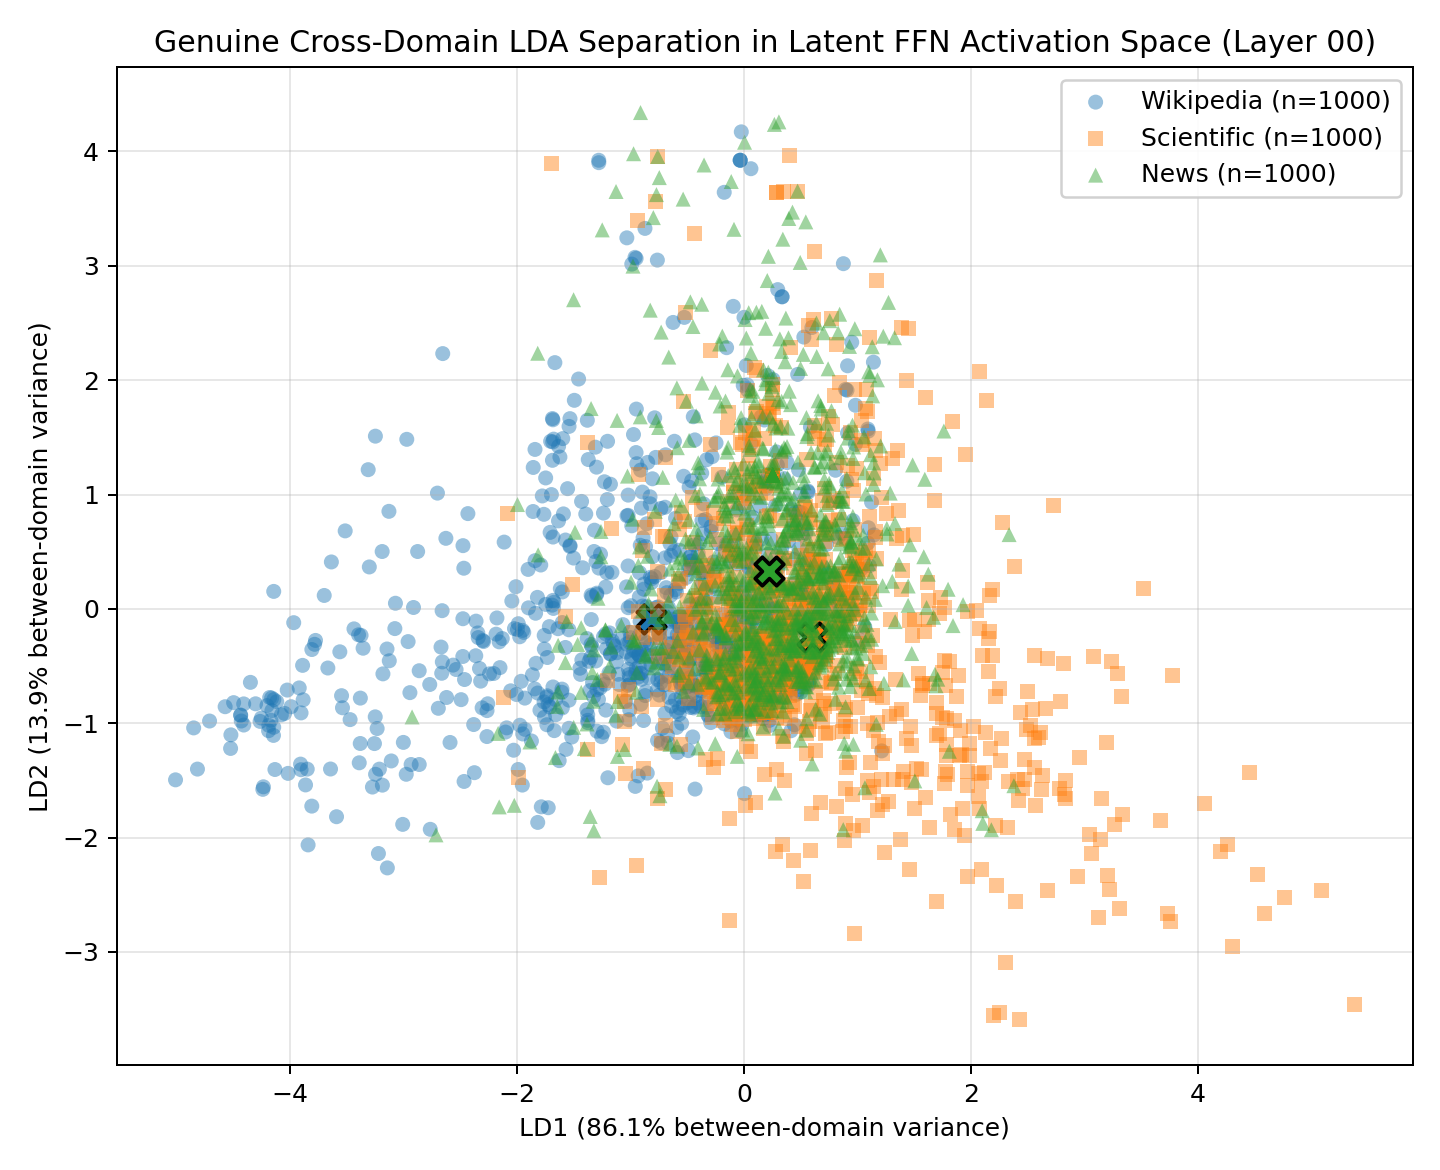
\includegraphics[width=0.82\textwidth]{figures/fig5_lda_domain_separation.png}
    \caption{Canonical Linear Discriminant Analysis projection of Layer~00 activations ($K = 8$ PCA subspace) across Wikipedia, ML-ArXiv Scientific, and AG-News ($n_g = 1{,}000$ per corpus). LD1 ($86.1\%$) separates Wikipedia from Scientific abstracts, while LD2 ($13.9\%$) shifts AG-News upward above an overlapping central core.}
    \label{fig:rq5_lda}
\end{figure}

\subsection{Interpretation: Covariance Heterogeneity and Discriminant Bias--Variance Trade-Off}

All four MANOVA criteria reject centroid equality across text domains ($\Lambda = 0.6939$, $F_{16, 5980} = 74.94$, $p = 7.86 \times 10^{-223}$). The two non-zero eigenvalues of $\mat{E}^{-1}\mat{H}$ are $\xi_1 = 0.3619$ and $\xi_2 = 0.0583$, yielding a bounded Roy statistic $\theta = \xi_1 / (1 + \xi_1) = 0.2657$ (with Heck parameters $s = 2$, $m = 2.5$, $\tilde{n} = 1{,}494$) and canonical variance shares of $86.13\%$ on LD1 and $13.87\%$ on LD2. Figure~\ref{fig:rq5_lda} illustrates this geometry: along LD1, Wikipedia tokens (centroid $\text{LD1} \approx -0.8$) separate from Scientific abstracts (centroid $\text{LD1} \approx +0.6$), while LD2 shifts AG-News tokens upward (centroid near $(+0.2, +0.35)$). Pairwise Hotelling's $T^2$ tests reflect these distances: Wikipedia diverges most sharply from Scientific text ($T^2 = 801.16$, $F = 99.79$), followed by Wikipedia versus News ($T^2 = 624.99$, $F = 77.85$), while Scientific and News centroids remain distinct ($T^2 = 283.17$, $F = 35.27$).

Simultaneously, Box's $M$ test rejects covariance equality ($M = 8{,}164.09$, $\chi^2_{72} = 8{,}133.62$, $p < 10^{-300}$), confirmed visually by the differentially oriented dispersion clouds in Figure~\ref{fig:rq5_lda}. This creates a classical methodological tension: pooled-covariance LDA assumes $\mat{\Sigma}_1 = \mat{\Sigma}_2 = \mat{\Sigma}_3$, whereas QDA accommodates class-specific dispersion. Empirically, 5-fold cross-validated LDA achieves $55.83\% \pm 0.96\%$ accuracy (a $+22.50$ percentage-point gain over the $33.33\%$ chance baseline), outperforming QDA ($51.57\% \pm 2.70\%$) with nearly three-fold lower fold-to-fold standard deviation. Two statistical factors explain this outcome:
\begin{enumerate}
    \item \textbf{Sensitivity of Box's $M$ to Kurtosis:} Because Box's $M$ compares log-determinants, heavy-tailed principal component scores derived from zero-inflated Layer~00 activations inflate test statistics even under moderate dispersion differences.
    \item \textbf{Estimation Variance in Quadratic Boundaries:} In $K = 8$ dimensions, LDA estimates a single pooled covariance matrix ($36$ free parameters), whereas QDA estimates three separate matrices ($108$ parameters). Under heavy tails and finite sample sizes ($n_g = 1{,}000$), inverting group covariance matrices $\mat{S}_g^{-1}$ amplifies outlier influence and degrades test classification relative to the constrained linear decision boundary.
\end{enumerate}

Unlike synthetic datasets with artificial clustering, genuine text tokens in early layers exhibit natural overlap due to shared syntactic structures, punctuation, and common vocabulary, explaining why realistic out-of-sample accuracy converges to approximately $55.8\%$ rather than an artificial ceiling.

% ------------------------------------------------------------------------------
% CHAPTER 5: CONCLUSION, LIMITATIONS, AND FUTURE WORK
% ------------------------------------------------------------------------------
\chapter{Conclusion, Methodological Limitations, and Future Work}

\section{Summary of Findings}

Evaluating \texttt{facebook/opt-125m} within applied multivariate statistics yields consistent empirical conclusions across all five research questions:
\begin{enumerate}
    \item \textbf{Non-Flat Sparsity Profile (RQ1):} Block-level profile analysis ($n = 40$) rejects depth-wise sparsity uniformity via Hotelling's $T^2$ ($p = 1.25 \times 10^{-57}$), Greenhouse--Geisser adjusted RM-ANOVA ($\hat{\epsilon} = 0.1253$, $p = 1.68 \times 10^{-46}$), and Friedman's rank test ($p = 5.99 \times 10^{-86}$). Sparsity increases from $88.96\%$ in Layer~00 to $98.77\%$ in Layer~03 before plateauing between $91.2\%\text{--}92.4\%$ in middle layers.
    \item \textbf{U-Shaped Co-Activation Dependence (RQ2):} Prevalence-filtered $\phi$-correlations show coordinated co-activation in Layer~00 ($\bar{\phi} = 0.0685$, $76.82\%$ positive pairs), disperse into near-zero correlations in Layers~01--10 ($\bar{\phi} \in [0.0026, 0.0071]$, with $122$ clusters at Layer~06), and re-couple in Layer~11 ($\bar{\phi} = 0.0391$, $94$ clusters).
    \item \textbf{Structured Effective Rank and Subspace Stability (RQ3):} Covariance PCA identifies severe low-rank collapse in Layers~00 and~02 ($\erank = 1.51$ and $1.86$), expanding to $\erank \approx 41\text{--}46$ across Layers~05--10, and re-compressing to $10.81$ at Layer~11. Split-half principal-angle cosines exceed $0.878$ at $K = 10$, confirming subspace stability.
    \item \textbf{Coupling Between Weight and Activation Ranks (RQ4):} SVD of actual parameter matrices confirms significant positive layer-wise correlation with empirical activation rank (Pearson $r = 0.799$, $p = 0.0018$; Spearman $\rho = 0.839$, $p = 0.00064$). Absolute activation rank ($\overline{\erank}_A = 26.38$) remains roughly 19 times smaller than mean weight effective rank ($\overline{\erank}_W = 500.53$), delineating structural weight capacity from dynamic ReLU compression.
    \item \textbf{Cross-Domain Sensitivity under Heteroscedasticity (RQ5):} Across genuine tokens from Wikipedia, ML-ArXiv, and AG-News at Layer~00, one-way MANOVA rejects equal centroids ($\Lambda = 0.6939$, $F_{16, 5980} = 74.94$, $p = 7.86 \times 10^{-223}$) and Box's $M$ rejects covariance equality ($\chi^2_{72} = 8{,}133.62$, $p < 10^{-300}$). Cross-validated LDA ($55.83\% \pm 0.96\%$) outperforms QDA ($51.57\% \pm 2.70\%$) due to lower parameter estimation variance.
\end{enumerate}

\section{Methodological Limitations}

Several statistical boundaries contextualise these findings:
\begin{itemize}
    \item \textbf{Finite Block Sample Size in RQ1:} Grouping tokens into contiguous 128-token blocks eliminates intra-sentence serial dependence at the expense of reducing profile sample size to $n = 40$ across $q = 12$ dimensions ($\mathrm{df}_2 = 29$ in Hotelling's $T^2$). Expanding to several hundred blocks would provide tighter simultaneous confidence bands and permit formal Mardia tests on $\vect{S}_b$.
    \item \textbf{Token Serial Autocorrelation in RQ2, RQ3, and RQ5:} Tokens extracted from the same text exhibit serial correlation. Consequently, nominal parametric $p$-values are anti-conservative; empirical effect sizes (Wilks' $\Lambda = 0.6939$, subspace stability $\bar{\rho}_{10}$, and cross-validated classification accuracy) serve as the primary criteria for statistical separation.
    \item \textbf{Distributional Departures from Normality:} Exact zeros and positive-tail skewness violate Gaussian assumptions in Box's $M$, Bartlett's sphericity test, and MLE factor analysis. While covariance PCA and Friedman's test are distribution-free, normal-theory likelihood ratio statistics are interpreted as approximate divergence measures rather than exact tail probabilities.
    \item \textbf{Layer Scope in Cross-Domain Testing:} Cross-domain MANOVA was conducted at Layer~00 ($K = 8$ PCs). Given that effective rank expands substantially in Layers~05--10, deeper layers may exhibit different domain separation and higher-dimensional covariance shifts.
\end{itemize}

\section{Directions for Future Research}

Four methodological extensions emerge from this work:
\begin{enumerate}
    \item \textbf{Multi-Sample Profile Analysis:} Computing block sparsity profiles $\vect{S}_b \in [0, 1]^{12}$ separately across Wikipedia, Scientific, and News text would enable full three-stage profile analysis testing parallelism, equal levels, and flatness across corpora.
    \item \textbf{Distribution-Free Multivariate Testing:} Incorporating permutation MANOVA, energy-distance tests, and regularised discriminant analysis (interpolating between LDA and QDA via shrinkage parameter $\gamma \in [0, 1]$) would directly accommodate zero-inflation and heteroscedasticity.
    \item \textbf{Zero-Inflated Latent Variable Frameworks:} Applying multivariate Tobit (censored Gaussian) or hurdle factor models would explicitly represent the discrete point mass at zero in~\eqref{eq:mixed_cdf}.
    \item \textbf{Comparative Architectural Studies:} Extending the protocol to smooth activation functions (GELU, SwiGLU) and larger models would assess whether early bottlenecking and positive weight--activation rank coupling persist when exact zero atoms are replaced by continuous near-zero tails.
\end{enumerate}

% ==============================================================================
% BIBLIOGRAPHY
% ==============================================================================
\begin{thebibliography}{9}
\addcontentsline{toc}{chapter}{Bibliography}

\bibitem{anderson2003introduction}
T.~W. Anderson, \emph{An Introduction to Multivariate Statistical Analysis}, 3rd~ed. Hoboken, NJ: John Wiley \& Sons, 2003.

\bibitem{box1949general}
G.~E.~P. Box, ``A general distribution theory for a class of likelihood criteria,'' \emph{Biometrika}, vol.~36, no.~3/4, pp.~317--346, 1949.

\bibitem{geva2021transformer}
M.~Geva, R.~Schuster, J.~Berant, and O.~Levy, ``Transformer feed-forward layers are key-value memories,'' in \emph{Proceedings of the 2021 Conference on Empirical Methods in Natural Language Processing (EMNLP)}, pp.~5484--5495, 2021.

\bibitem{hardle2019applied}
W.~K. H{\"a}rdle and L.~Simar, \emph{Applied Multivariate Statistical Analysis}, 5th~ed. Cham: Springer, 2019.

\bibitem{johnson2014applied}
R.~A. Johnson and D.~W. Wichern, \emph{Applied Multivariate Statistical Analysis}, 6th~ed. Harlow: Pearson Education, 2014.

\bibitem{li2023emergence}
Z.~Li, C.~Wang, Y.~Gu, C.~Liu, and J.~Chen, ``On emergence of activation sparsity in trained transformers,'' in \emph{International Conference on Learning Representations (ICLR)}, 2023.

\bibitem{mardia1970measures}
K.~V. Mardia, ``Measures of multivariate skewness and kurtosis with applications,'' \emph{Biometrika}, vol.~57, no.~3, pp.~519--530, 1970.

\bibitem{rao1973linear}
C.~R. Rao, \emph{Linear Statistical Inference and Its Applications}, 2nd~ed. New York: John Wiley \& Sons, 1973.

\bibitem{roy2007effective}
O.~Roy and M.~Vetterli, ``The effective rank: A measure of effective dimensionality,'' in \emph{15th European Signal Processing Conference (EUSIPCO)}, pp.~606--610, 2007.

\end{thebibliography}

% ==============================================================================
% APPENDIX
% ==============================================================================
\appendix
\chapter{Layer-by-Layer RQ4 SVD Spectral Metrics}
\label{app:rq4_details}

Table~\ref{tab:app_rq4_layer_data} presents the complete layer-wise empirical activation effective dimensionality metrics alongside singular value decomposition statistics for the actual \texttt{facebook/opt-125m} \texttt{fc1} ($3072 \times 768$) and \texttt{fc2} ($768 \times 3072$) weight matrices.

\begin{table}[htbp]
    \centering
    \caption{Layer-by-layer comparison of empirical activation effective dimensionality and actual \texttt{facebook/opt-125m} FFN weight matrix spectral dimensionality (RQ4). All parameter matrices possess full algebraic rank $768$.}
    \label{tab:app_rq4_layer_data}
    \small
    \setlength{\tabcolsep}{5pt}
    \begin{tabular}{@{}l r r r r r r r@{}}
        \toprule
        \textbf{Layer} & \textbf{Act.\ $\erank$} & \textbf{Act.\ $\PR$} & \textbf{\texttt{fc1} $\erank$} & \textbf{\texttt{fc1} $\PR$} & \textbf{\texttt{fc2} $\erank$} & \textbf{\texttt{fc2} $\PR$} & \textbf{Mean Wt.\ $\erank$} \\
        \midrule
        Layer 00 &  1.51 &  1.12 & 232.38 &  28.63 & 509.70 & 354.46 & 371.04 \\
        Layer 01 & 13.06 &  3.89 & 416.92 & 124.56 & 548.55 & 361.58 & 482.74 \\
        Layer 02 &  1.86 &  1.20 & 310.96 &  52.73 & 546.44 & 380.46 & 428.70 \\
        Layer 03 &  7.72 &  2.45 & 396.26 & 114.55 & 526.35 & 383.11 & 461.31 \\
        Layer 04 & 12.19 &  3.51 & 483.45 & 179.50 & 568.10 & 444.60 & 525.78 \\
        Layer 05 & 46.36 & 31.40 & 518.30 & 211.76 & 551.90 & 420.84 & 535.10 \\
        Layer 06 & 45.53 & 29.86 & 516.51 & 206.00 & 537.98 & 396.21 & 527.24 \\
        Layer 07 & 45.98 & 30.99 & 515.41 & 207.58 & 561.58 & 438.15 & 538.49 \\
        Layer 08 & 46.10 & 31.42 & 519.23 & 208.79 & 565.71 & 442.29 & 542.47 \\
        Layer 09 & 44.03 & 29.64 & 504.54 & 202.79 & 580.40 & 469.39 & 542.47 \\
        Layer 10 & 41.43 & 27.64 & 490.30 & 185.51 & 584.32 & 470.53 & 537.31 \\
        Layer 11 & 10.81 &  3.38 & 477.79 & 168.85 & 549.64 & 303.71 & 513.72 \\
        \midrule
        \textbf{Mean} & \textbf{26.38} & \textbf{16.38} & \textbf{448.50} & \textbf{150.94} & \textbf{552.56} & \textbf{405.45} & \textbf{500.53} \\
        \bottomrule
    \end{tabular}
\end{table}

\end{document}
